\documentclass[a4paper,12pt]{article}

\usepackage{microtype}
\usepackage{graphicx}
\usepackage{wrapfig}
\usepackage{enumitem}
\usepackage{fancyhdr}
\usepackage{amsmath}
\usepackage{index}
\usepackage{float}


\begin{document}
\title{CSE 802 Homework 1}
\author{By Abhiram Durgaraju}
\date{February 2, 2020}
\maketitle
\pagestyle{empty}
\pagebreak
\section*{Problem 1:}
\subsection*{Part a:}
The mean pattern vector or centroid for each class was calculated in MATLAB. They are shown below:\\ \\
Class 1 centroid: 
\newline
[7.3333, 9.2083, 8.1875, 5.9375, 9.3125, 11.4375, 3.1458, 3.7708]
\newline
Class 2 centroid:
\newline
[5.6666, 5.1250, 5.3750, 6.0625, 4.6458, 4.6041, 7.8958, 9.4375]
\newline
Class 3 centroid:
\newline
[7.3125, 7.2083, 6.7291, 5.9791, 5.3333, 5.4791, 3.7291, 4.2083]
\newline
Class 4 centroid:
\newline
[8.2708, 8.0833, 7.2500, 6.0000, 9.1875, 9.6250, 6.4166, 7.4375]
\\
\subsection*{Part b:}
Using Euclidean distance, the pattern vector that is farthest from the class mean was  found using MATLAB, shown below: \\ \\
Class 1: \newline
[12     9     7    13    13     8     3     2] 
\newline
Class 2: \newline
[6     6     4    16     4     4     4    14]
\newline
Class 3: \newline
[6     6     5     5     4     4     0     2]
\newline
Class 4: \newline
[2     3    12     7     8    12     7     8] 
\newline

\subsection*{Part c:}
It is difficult to distinguish between the 4 classes using histograms with frequencies overlapped on top of each other. So, to analyze the features and their usefulness, I opted to visualizing them side-by-side using subplots in MATLAB. For all 8 features, I have computed the overlapped histogram frequencies and the subplots. They are shown below:
\pagebreak

\begin{figure}[H]
\centering
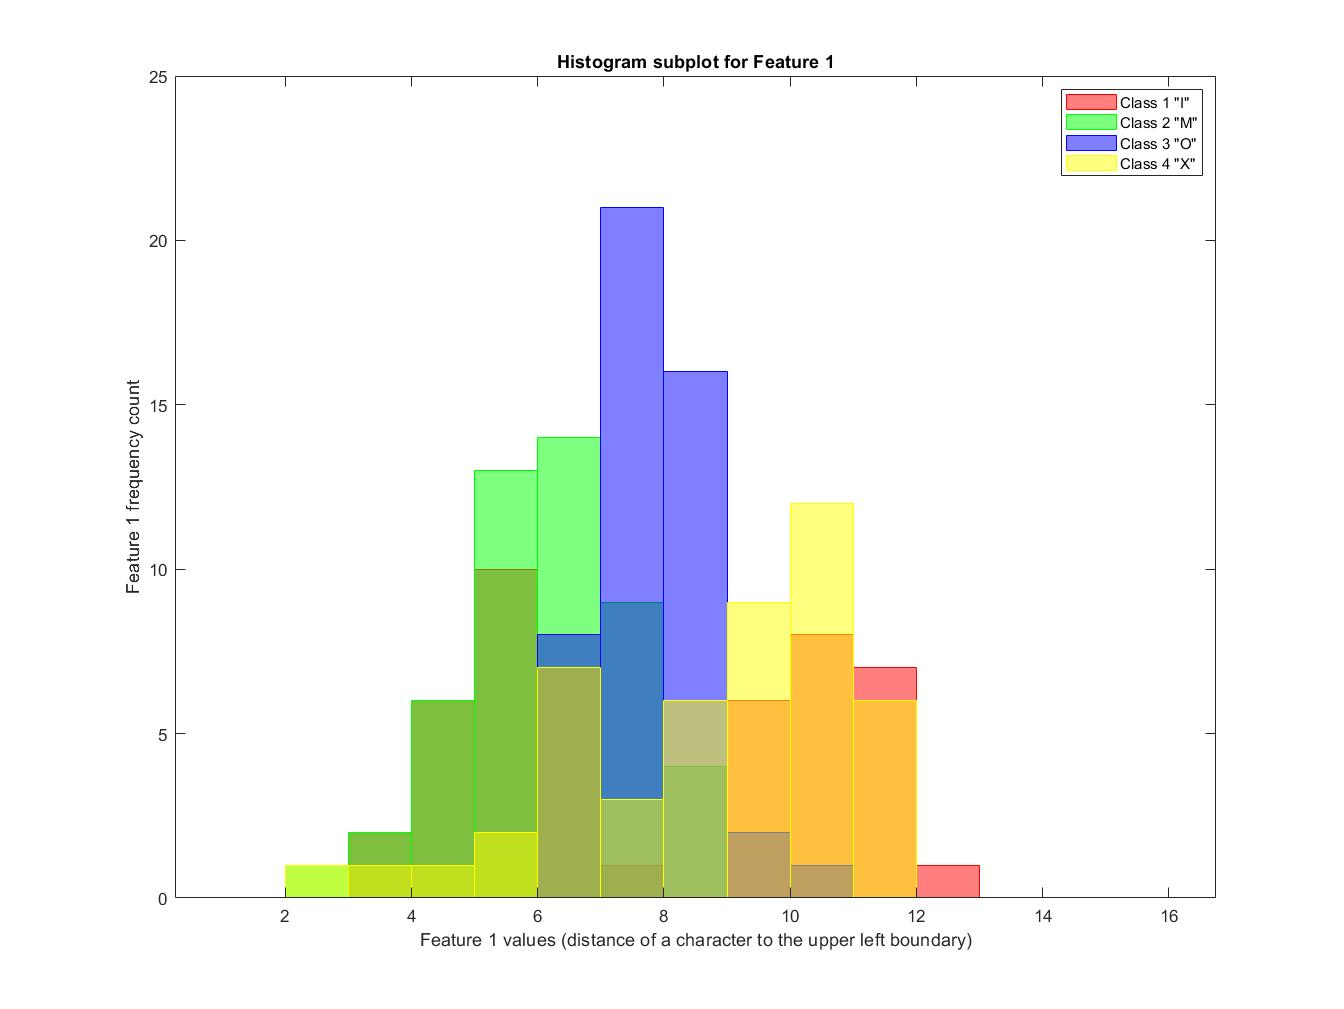
\includegraphics[scale=0.3]{q1pc_1.jpg}
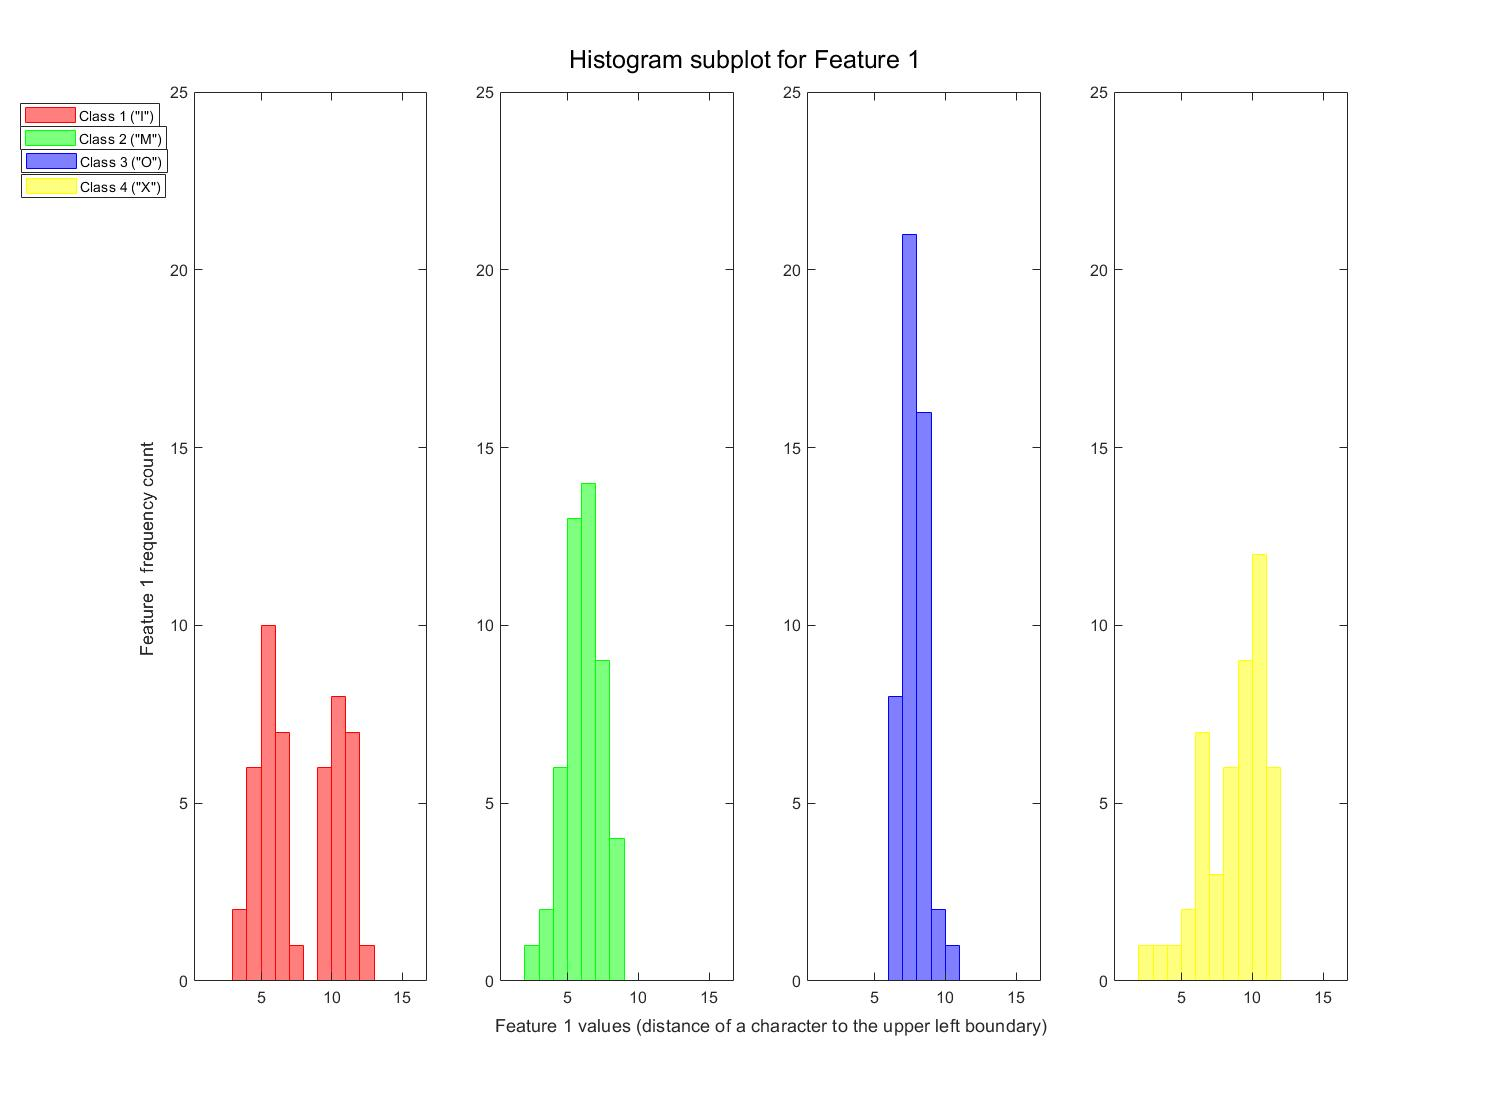
\includegraphics[scale=0.3]{q1pcs_1.jpg}
\end{figure}
\pagebreak
\begin{figure}[H]
\centering
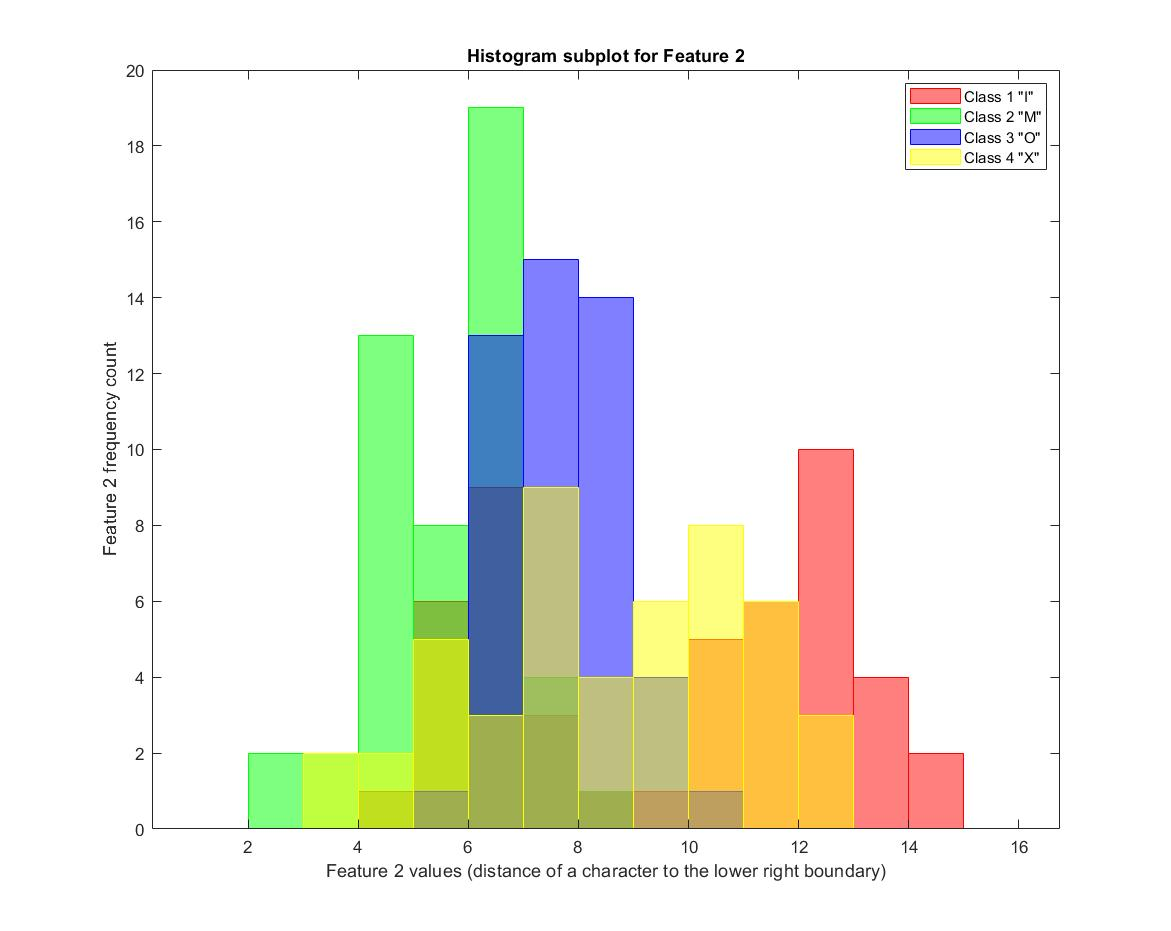
\includegraphics[scale=0.3]{q1pc_2.jpg}
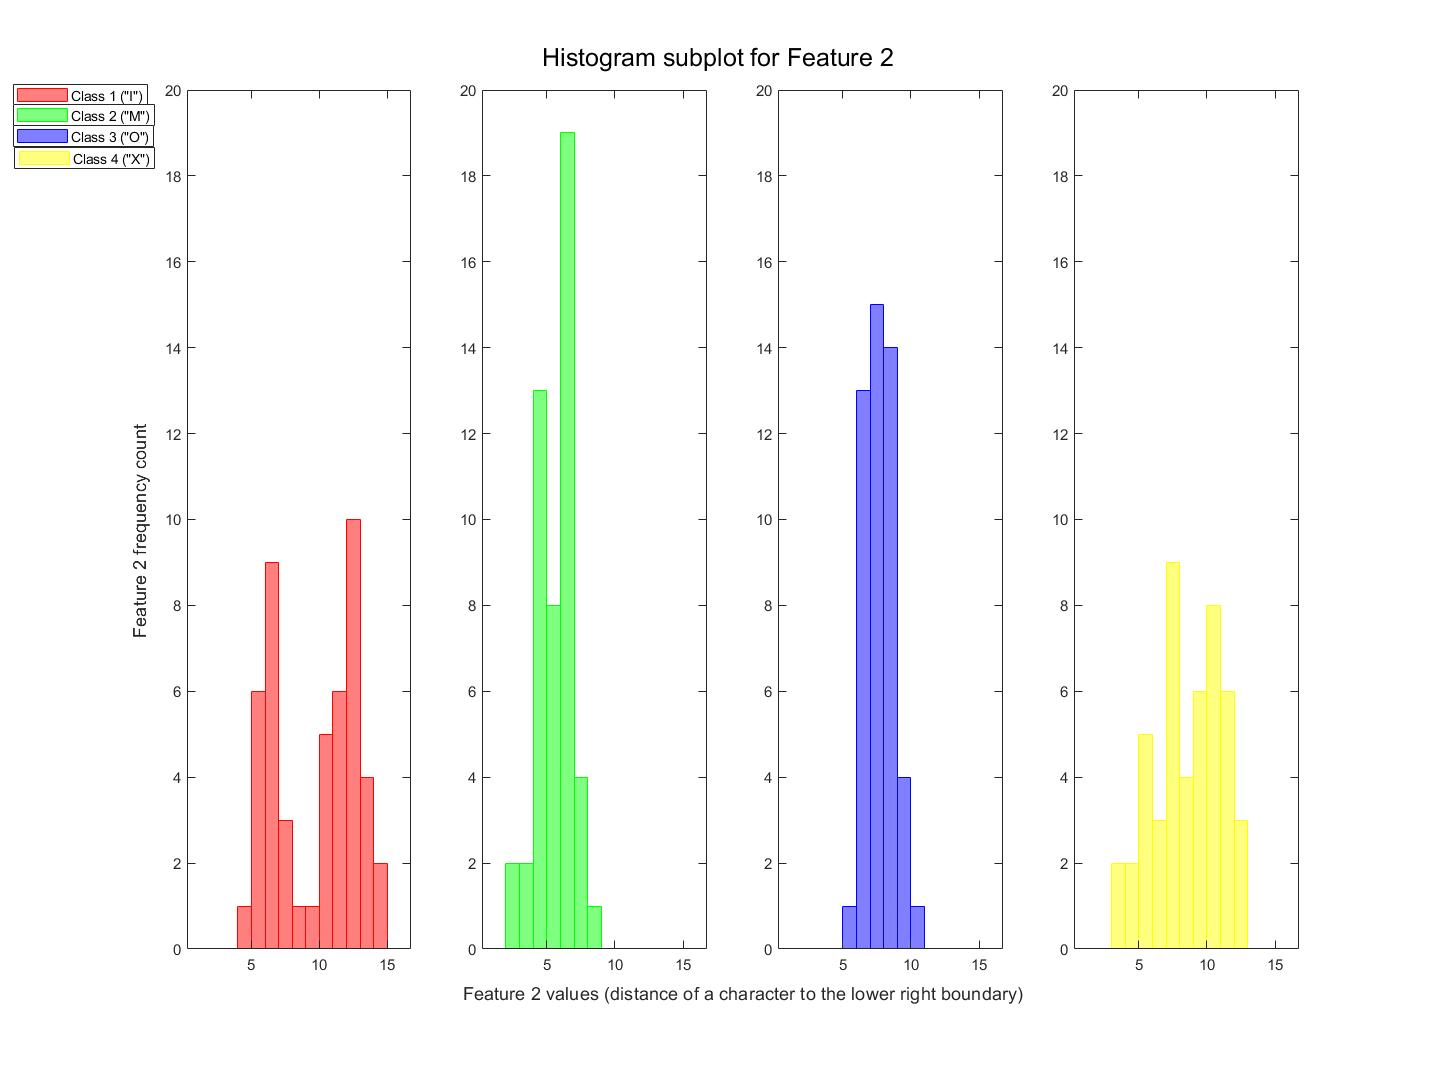
\includegraphics[scale=0.3]{q1pcs_2.jpg}
\end{figure}
\pagebreak
\begin{figure}[H]
\centering
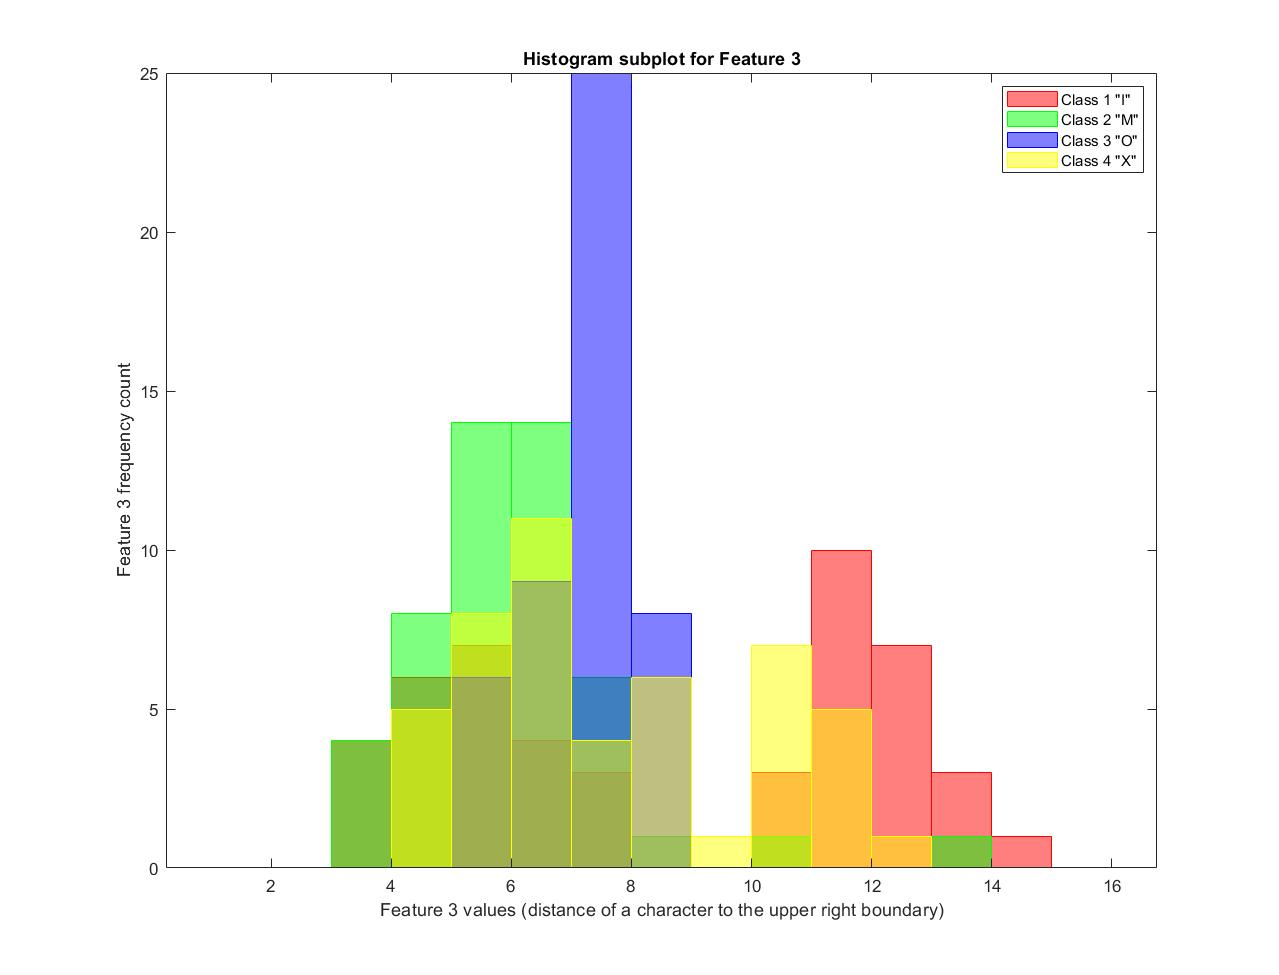
\includegraphics[scale=0.3]{q1pc_3.jpg}
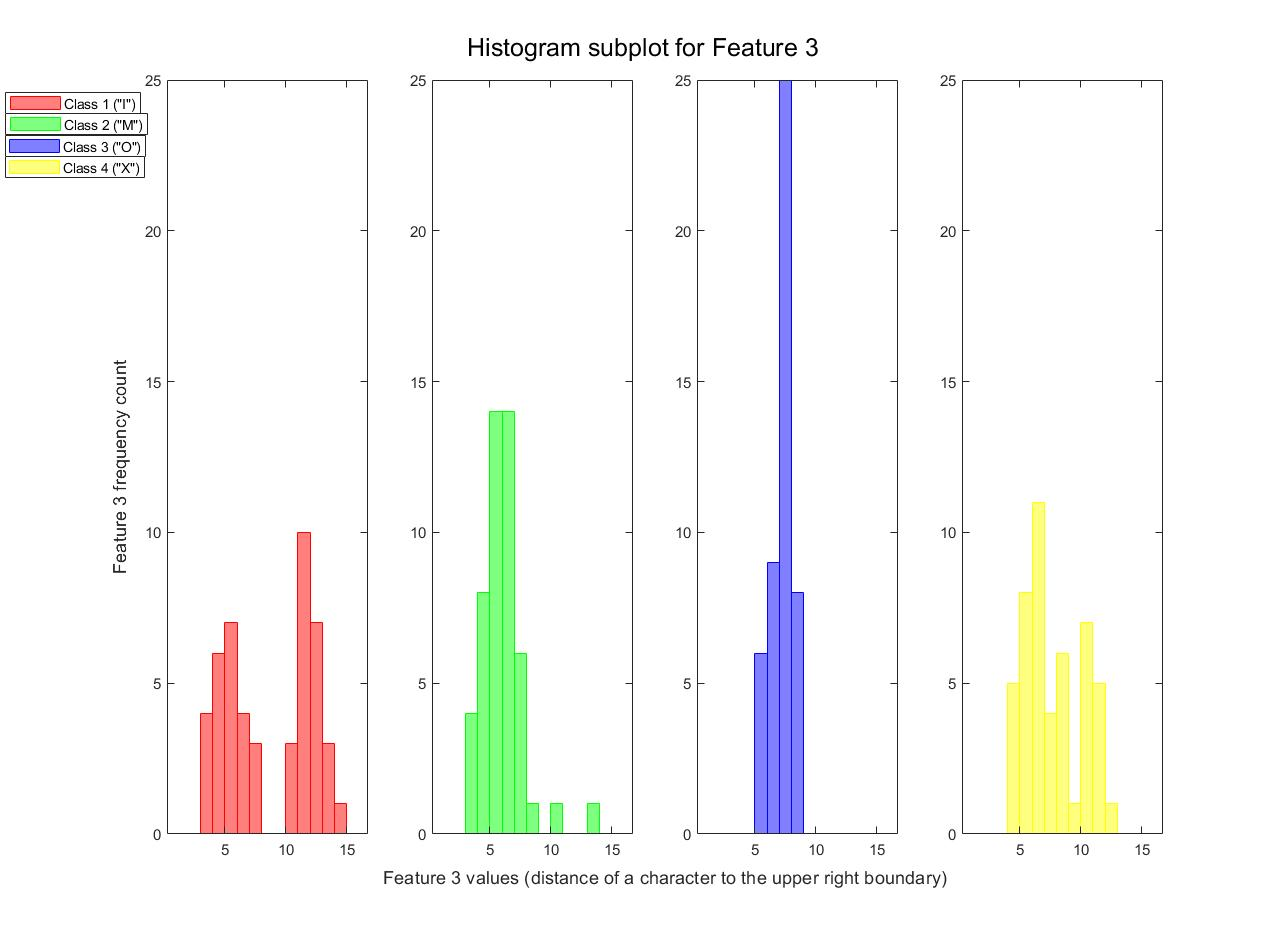
\includegraphics[scale=0.3]{q1pcs_3.jpg}
\end{figure}
\pagebreak
\begin{figure}[H]
\centering
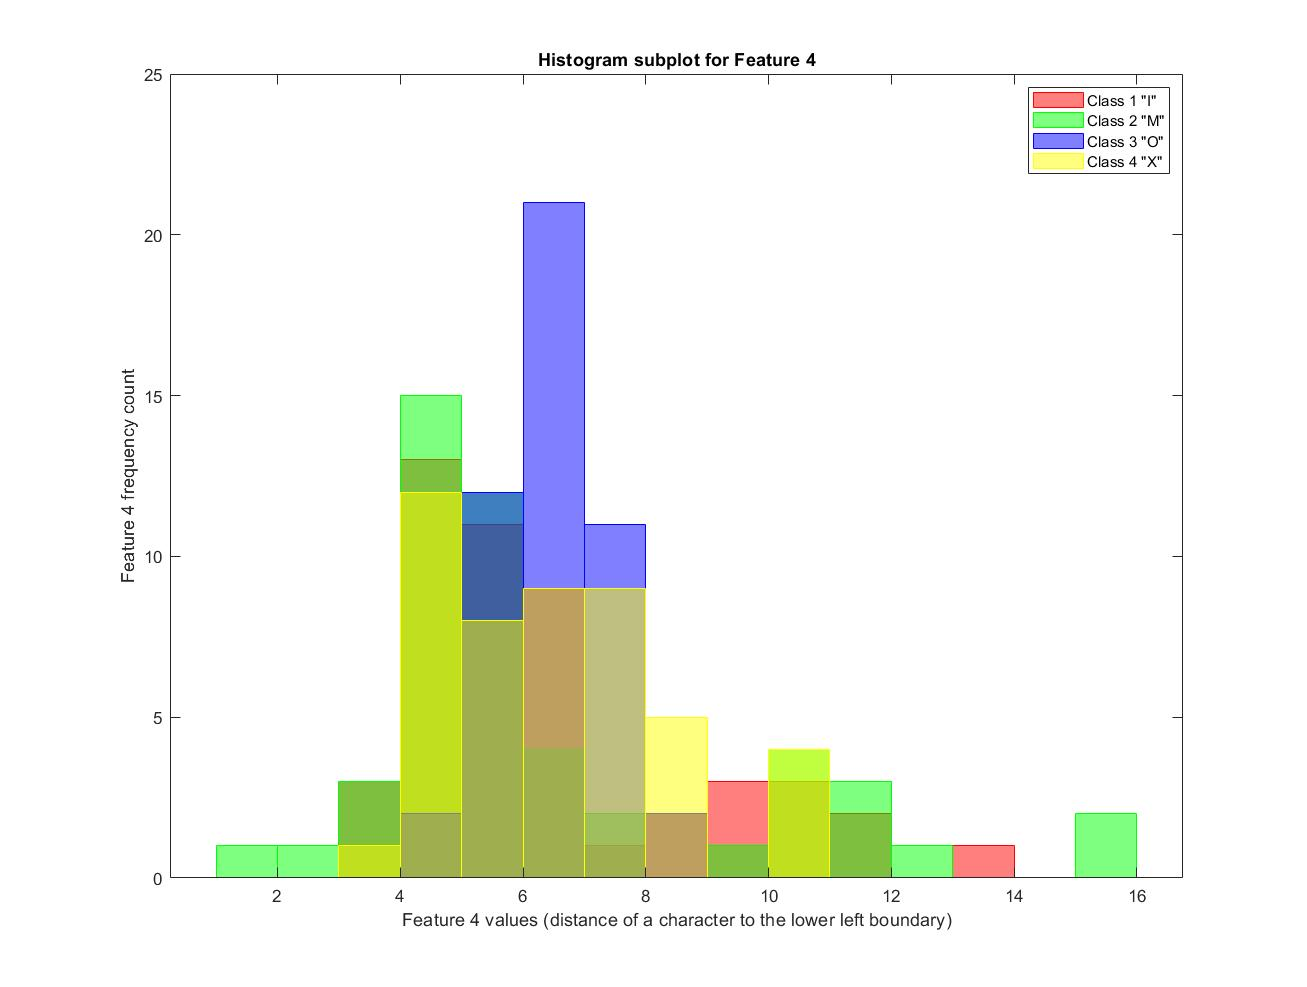
\includegraphics[scale=0.3]{q1pc_4.jpg}
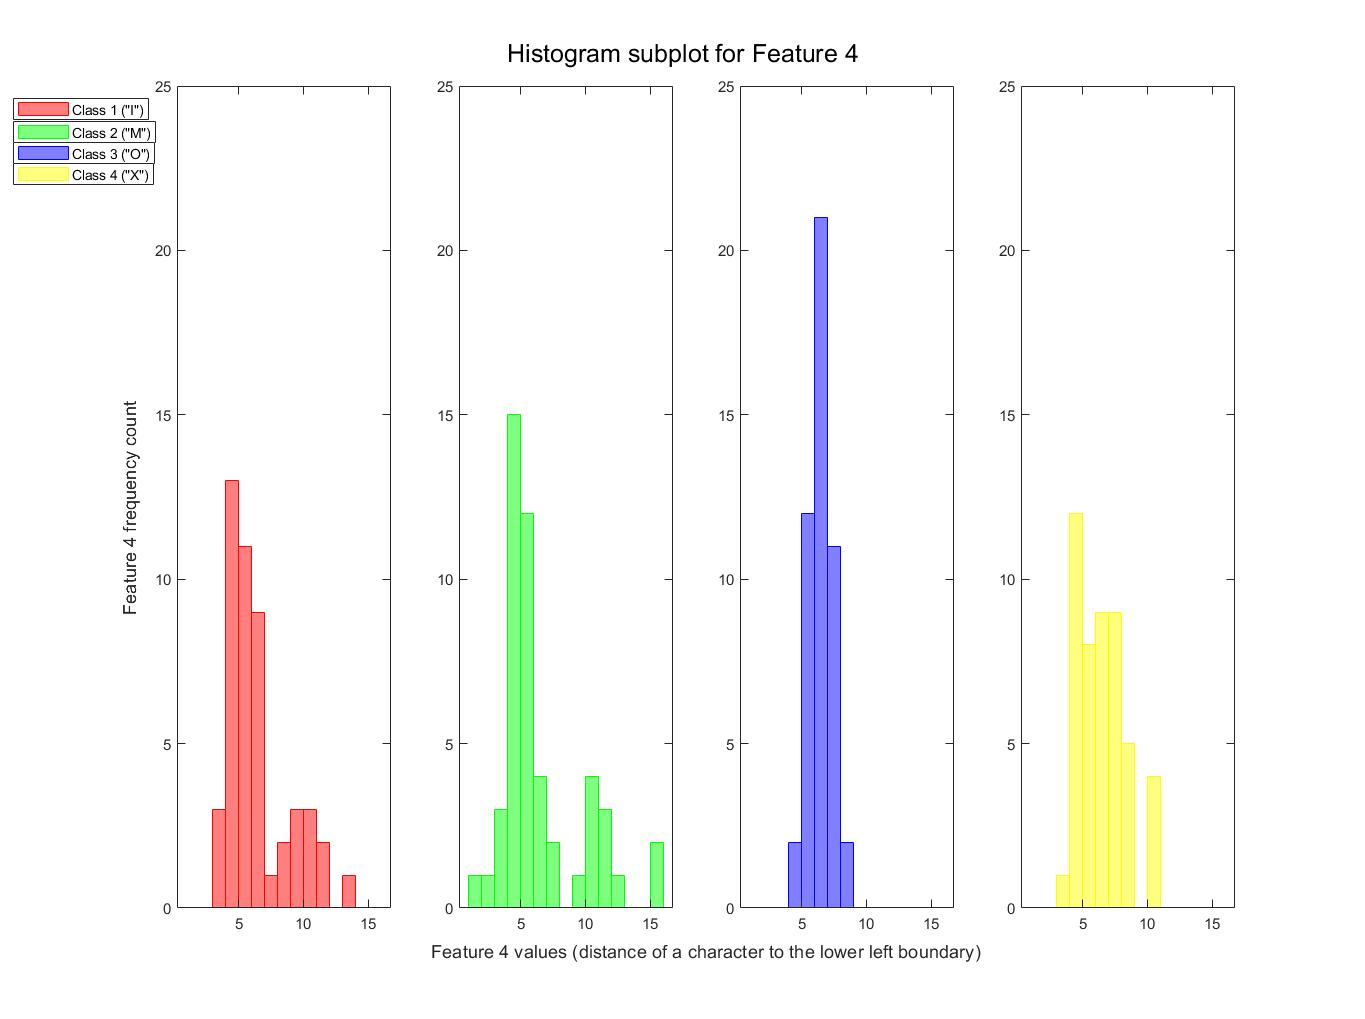
\includegraphics[scale=0.3]{q1pcs_4.jpg}
\end{figure}
\pagebreak
\begin{figure}[H]
\centering
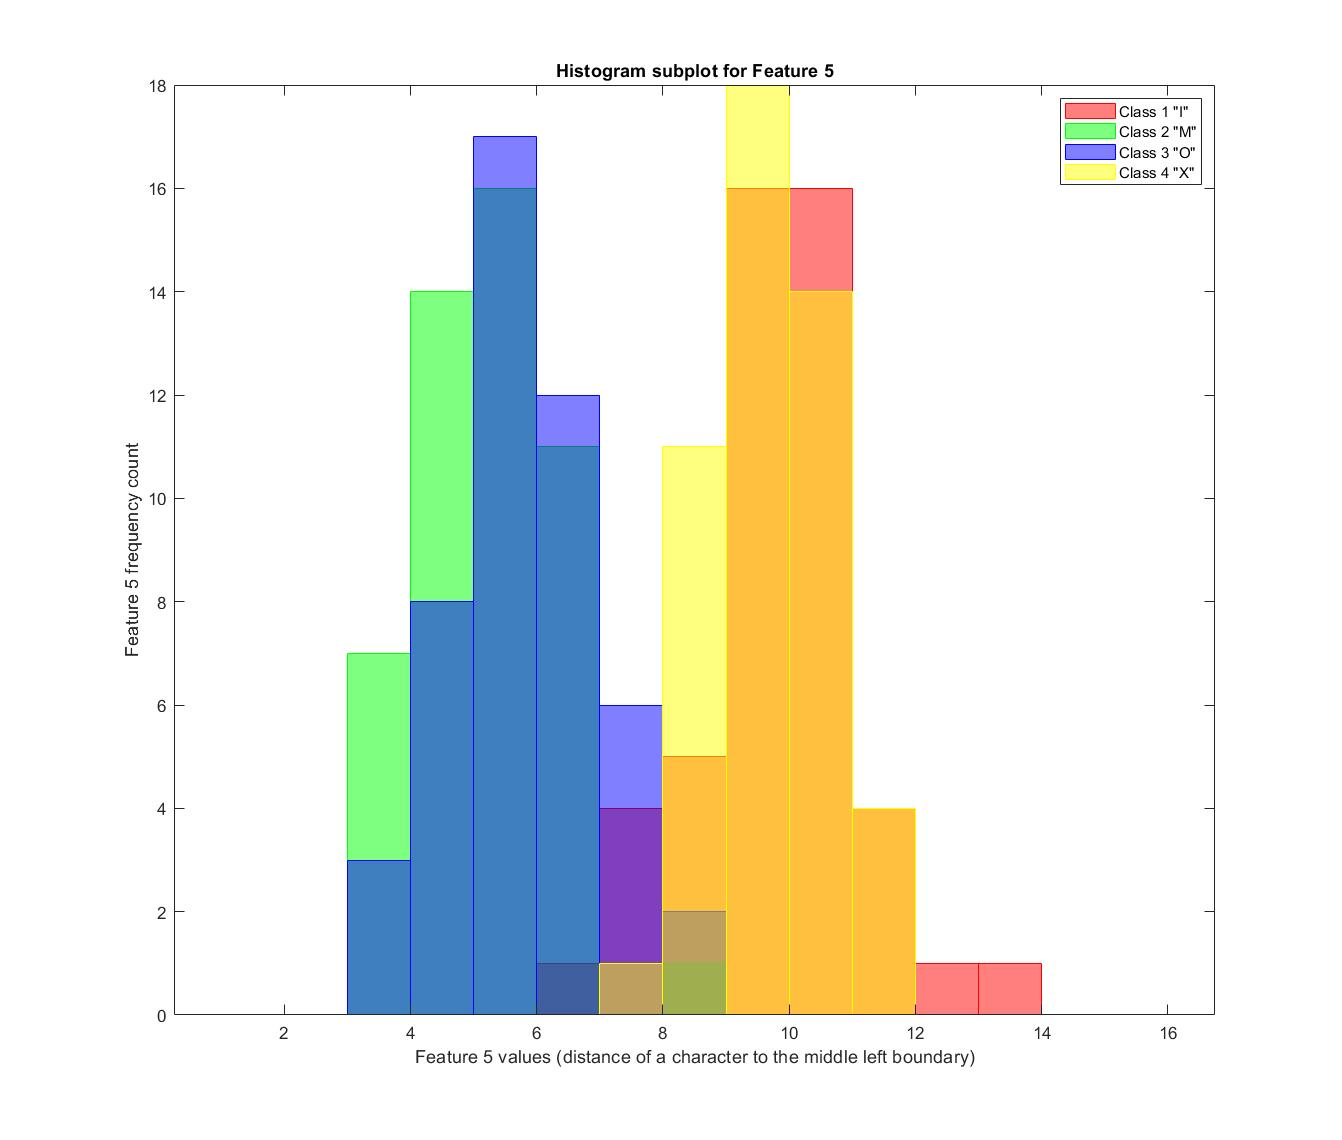
\includegraphics[scale=0.3]{q1pc_5.jpg}
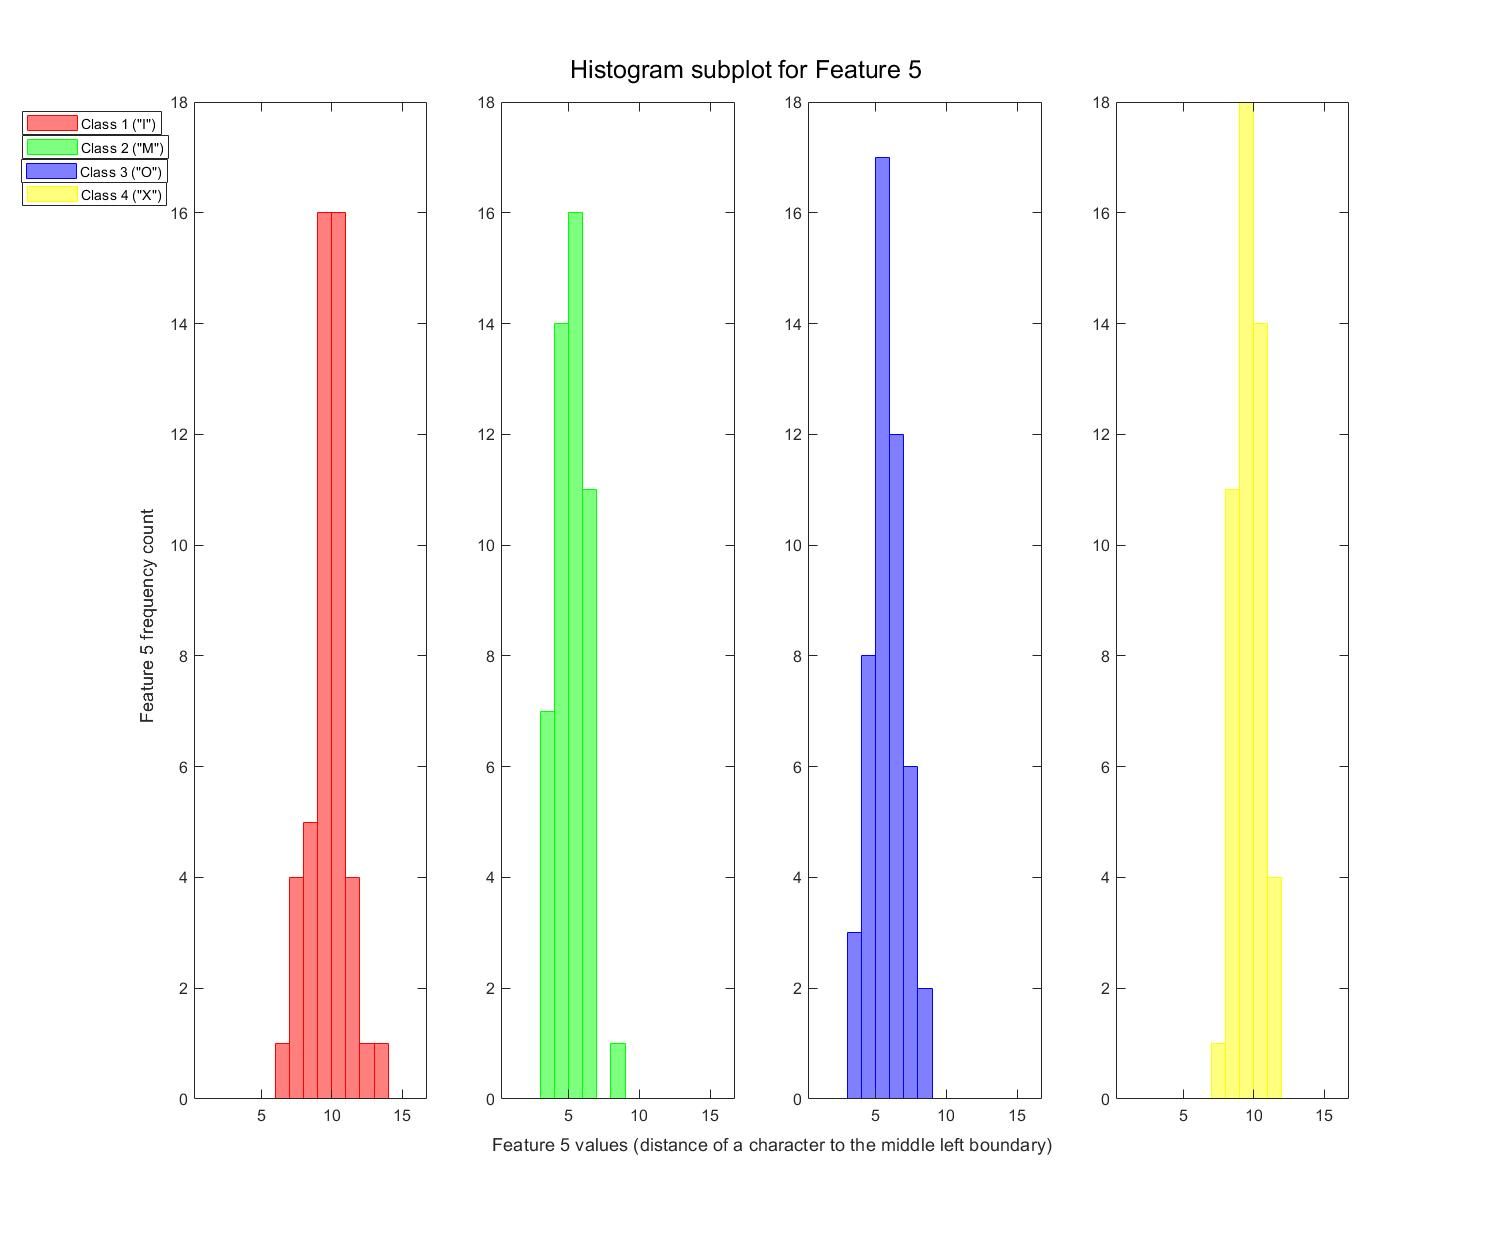
\includegraphics[scale=0.3]{q1pcs_5.jpg}
\end{figure}
\pagebreak
\begin{figure}[H]
\centering
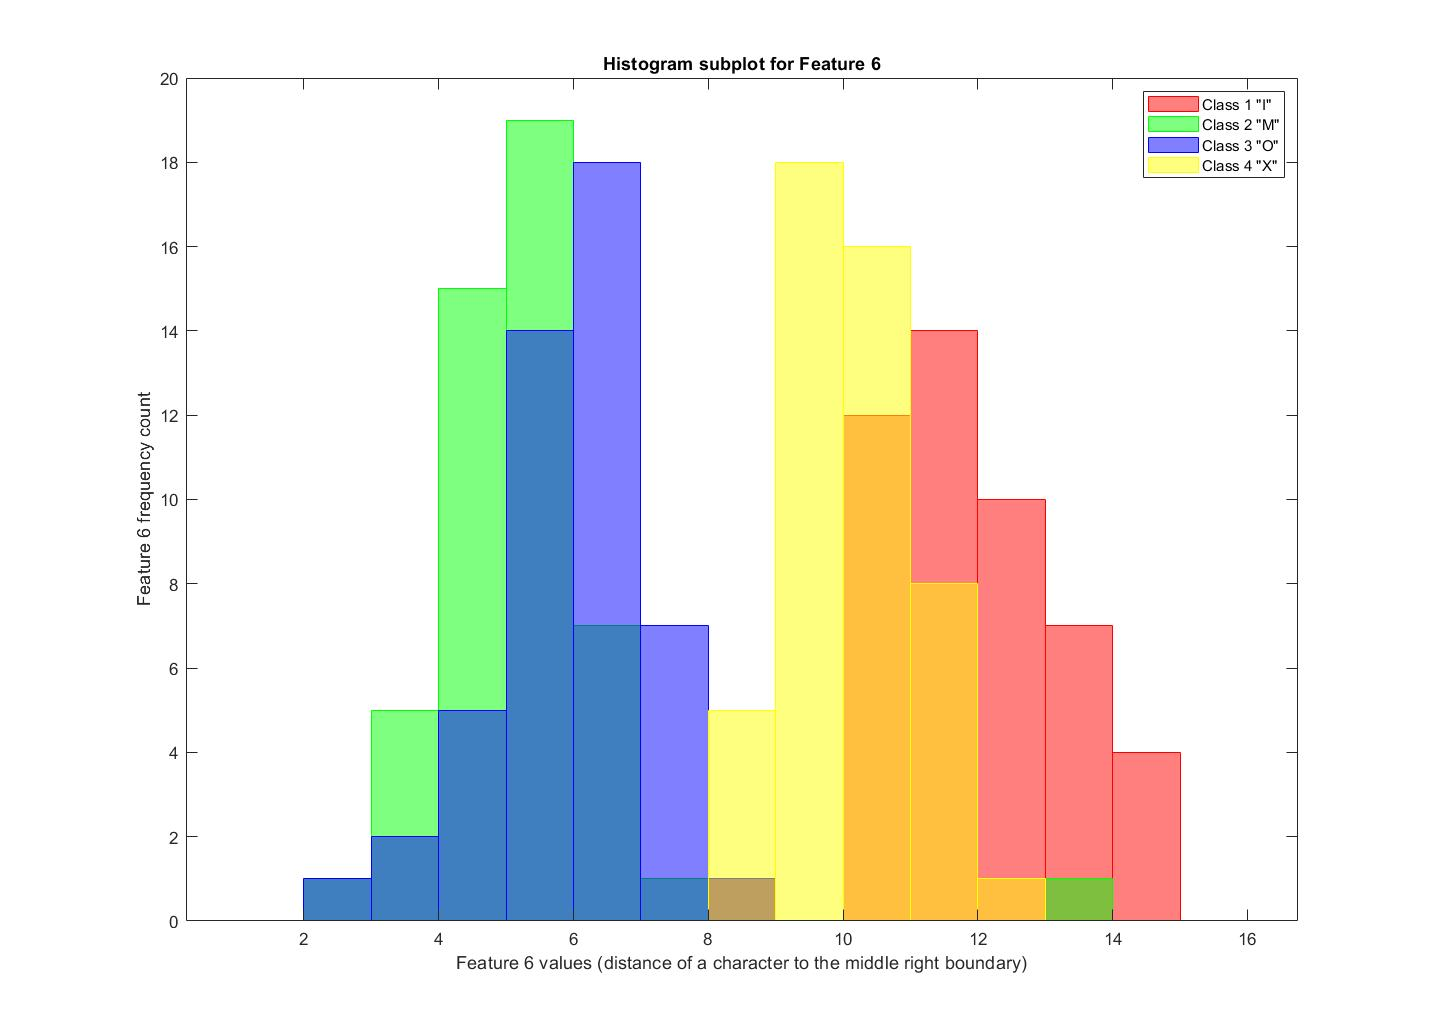
\includegraphics[scale=0.3]{q1pc_6.jpg}
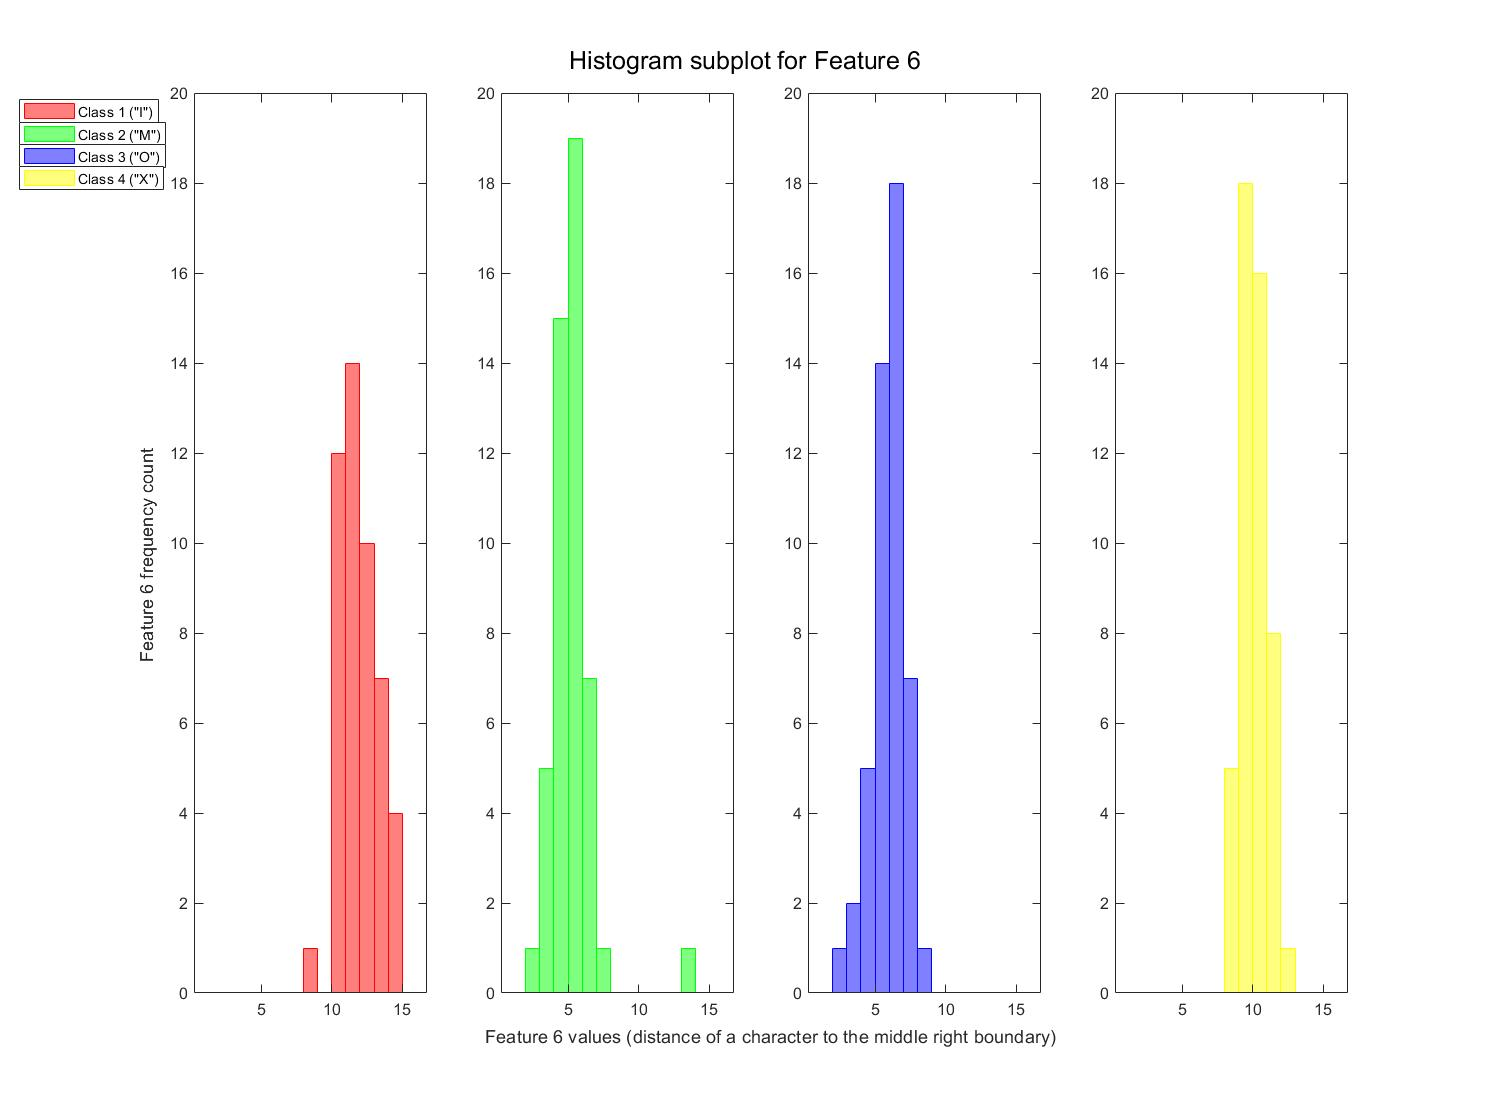
\includegraphics[scale=0.3]{q1pcs_6.jpg}
\end{figure}
\pagebreak
\begin{figure}[H]
\centering
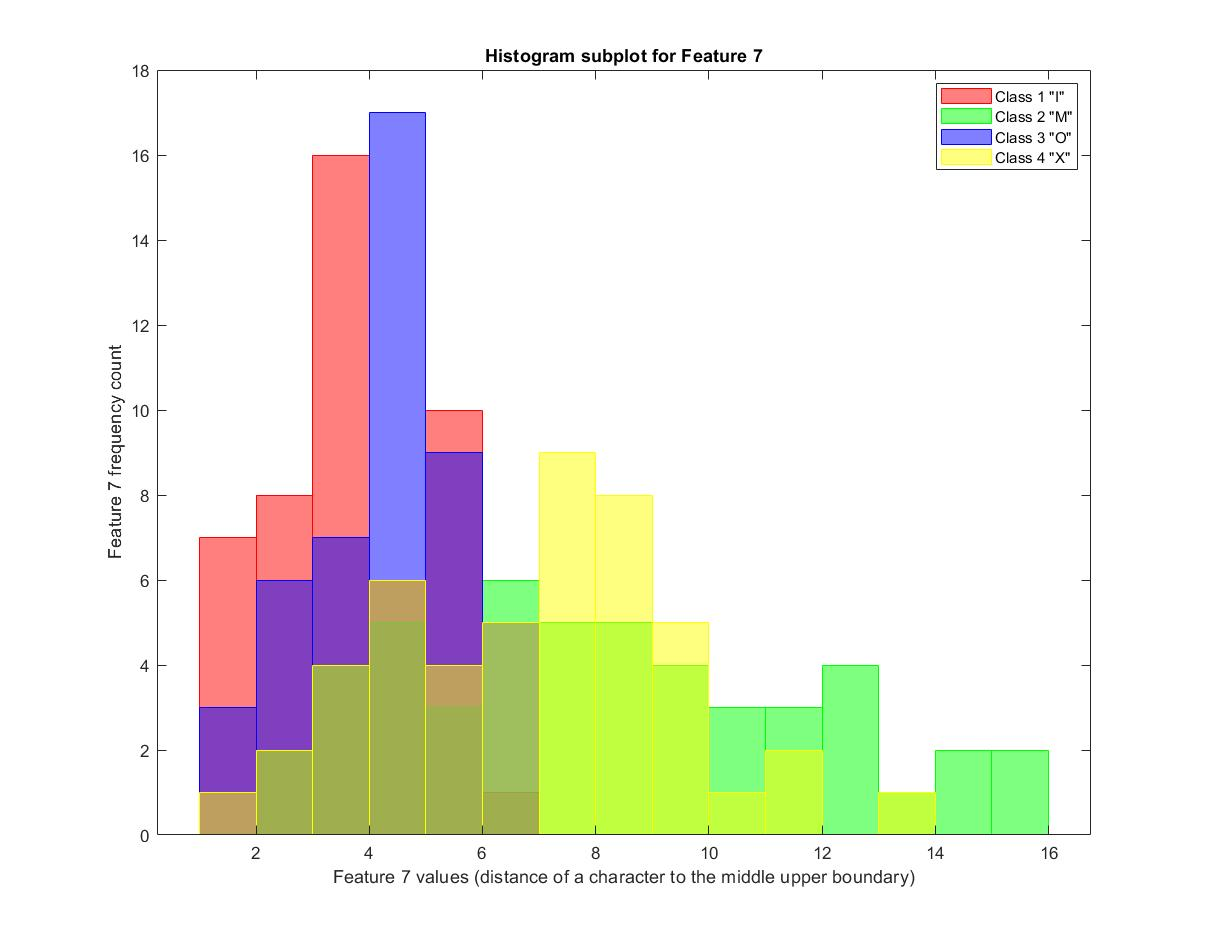
\includegraphics[scale=0.3]{q1pc_7.jpg}
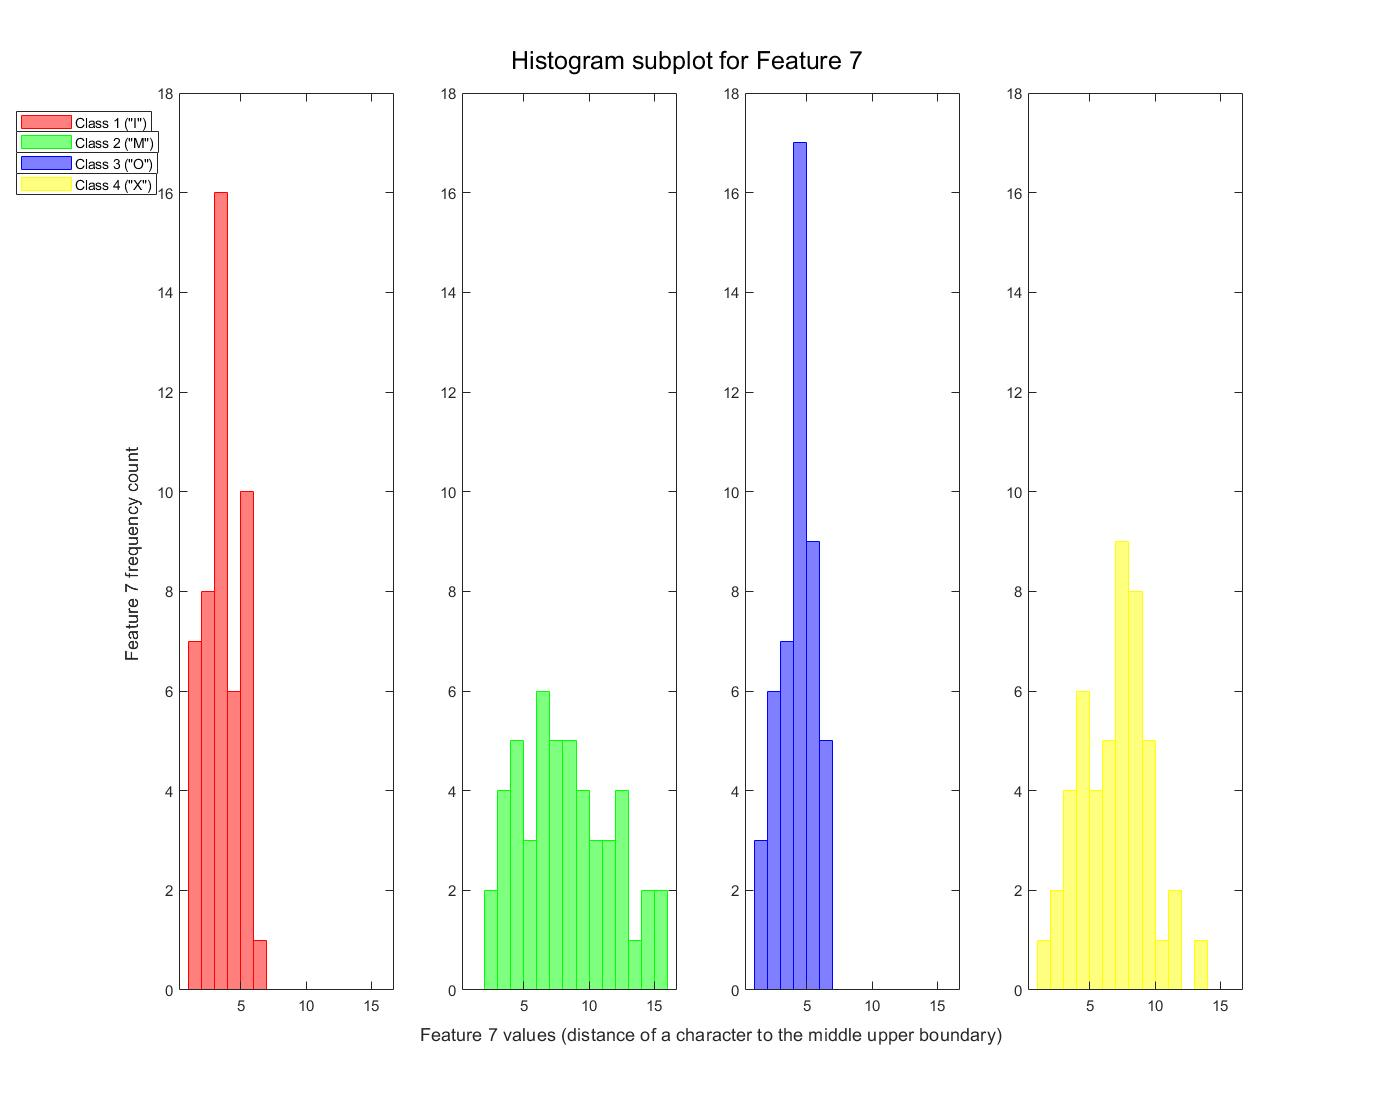
\includegraphics[scale=0.3]{q1pcs_7.jpg}
\end{figure}
\pagebreak
\begin{figure}[H]
\centering
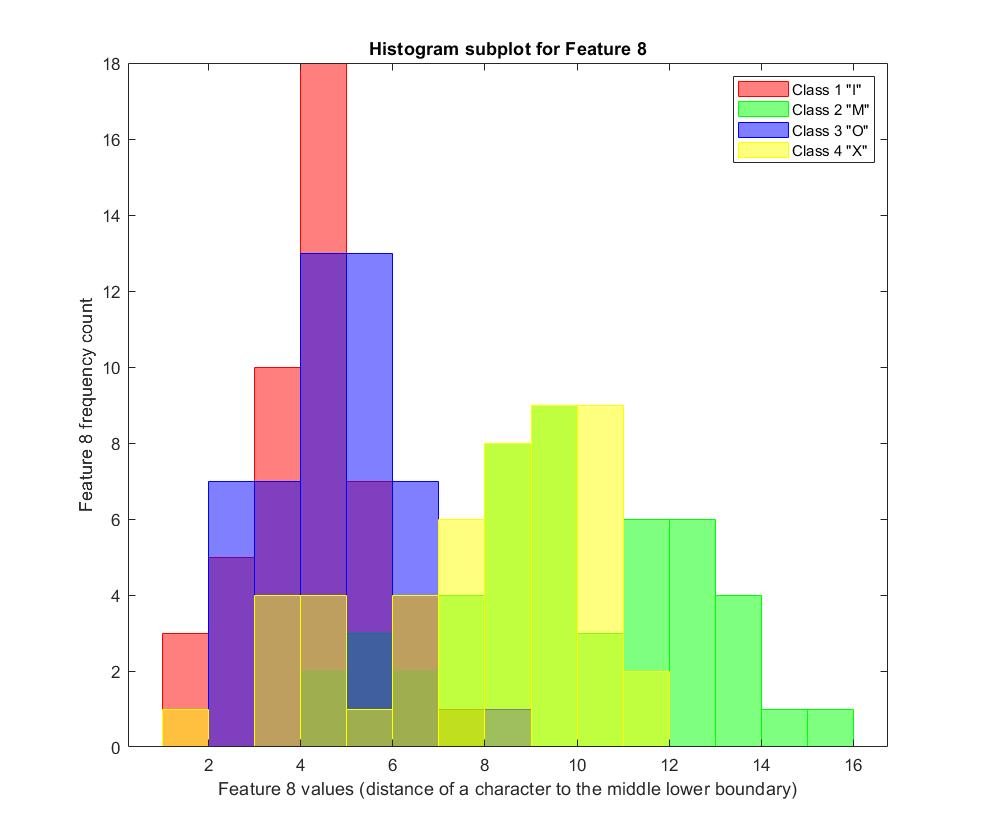
\includegraphics[scale=0.3]{q1pc_8.jpg}
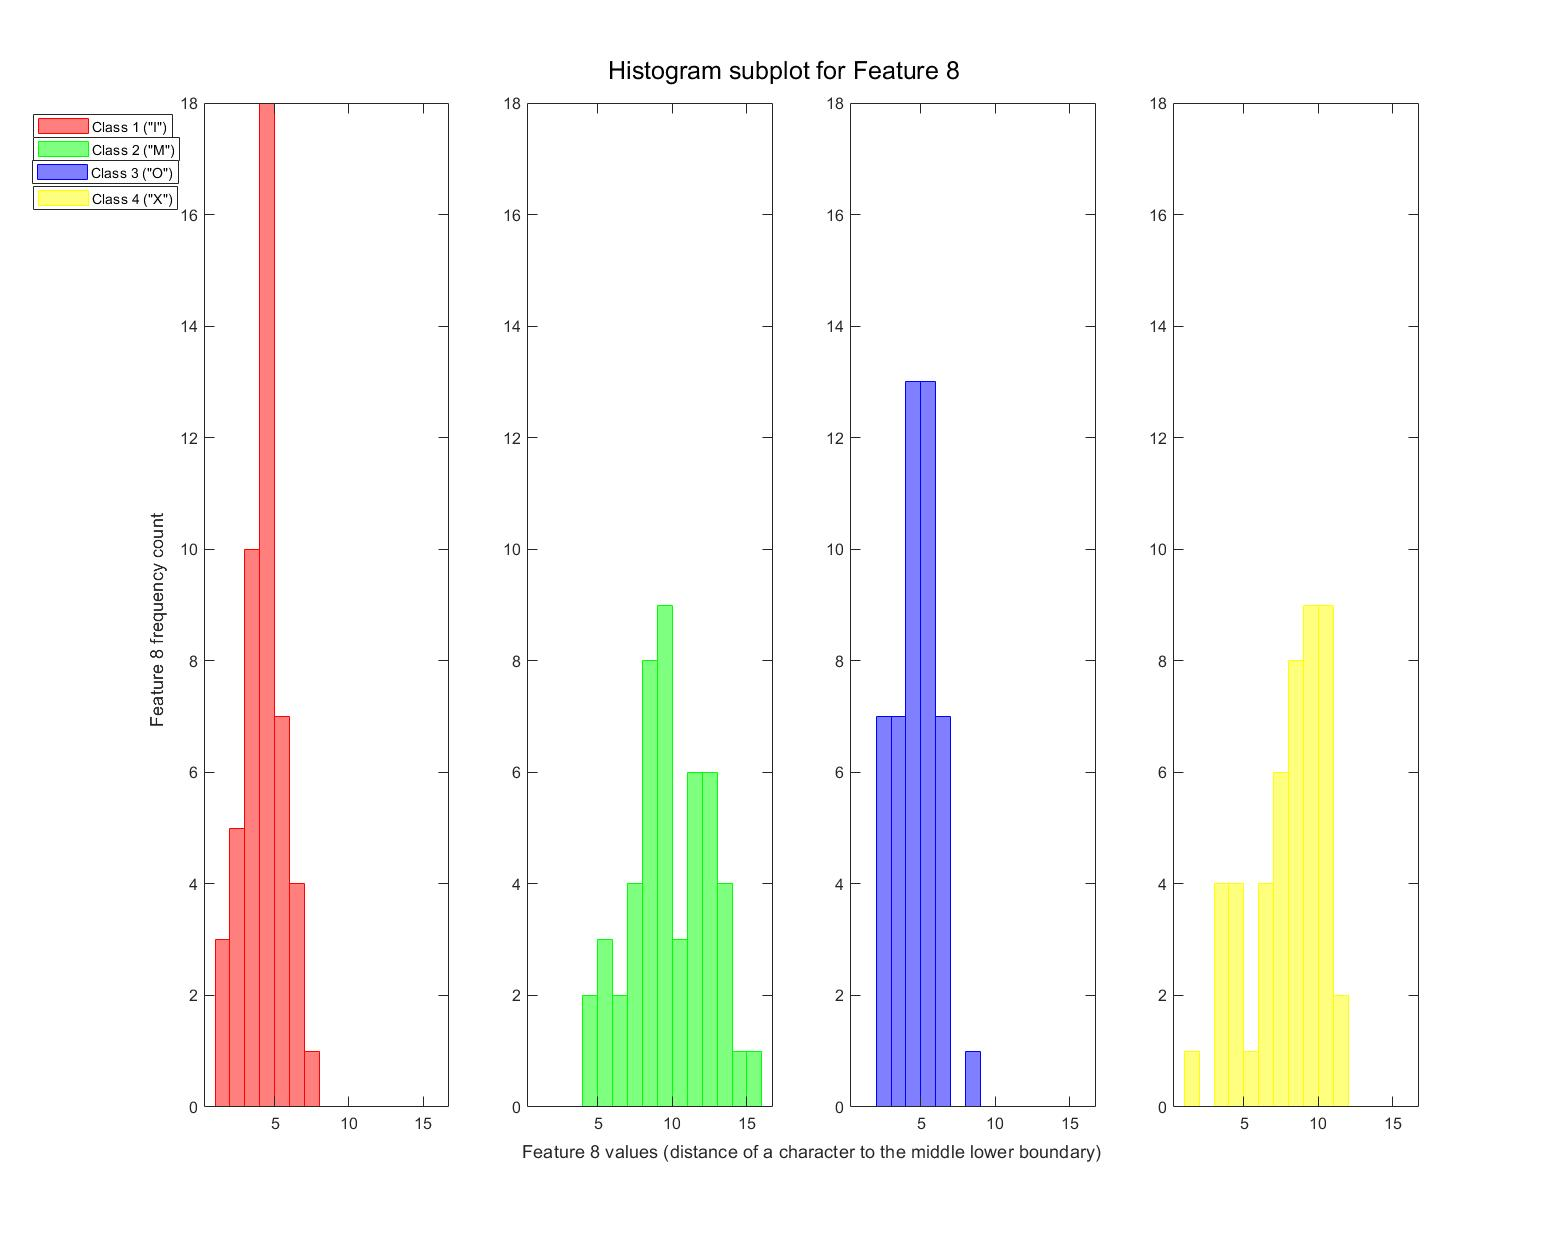
\includegraphics[scale=0.3]{q1pcs_8.jpg}
\end{figure}

No single feature is perfect for distinguishing between all 4 classes, as all of the features have some degree of overlap in feature values for a given feature. Useful features are those with the least overlap between classes, i.e they have the greatest inter-class variability.\\
Feature 2 is useful for this exact reason: Relative to othe classes, class 1 has more patterns with feature values between 13-15; class 2 has many patterns with feature values between 2-5; class 3 has many patterns with feature values between 7-8; class 4 has many patterns with feature values between 9-10. \\
Feature 5 is useful for distinguishing between class 2 and class 4: class 2 has many patterns with feature values between 3-7; class 4 has many paterns with feature values between 7-12. \\ \\
Class 1 and class 3 are likely to overlap with each other to a great extent. This is particulary clear when looking at features 7 and 8; For these two features, class 1 and class 3 have low inter-class variability. Feature 3 also tells a similar story, but with slightly larger inter-class variability between class 1 and class 3. \\

\subsection*{Part d:}
\begin{figure}[H]
\centering
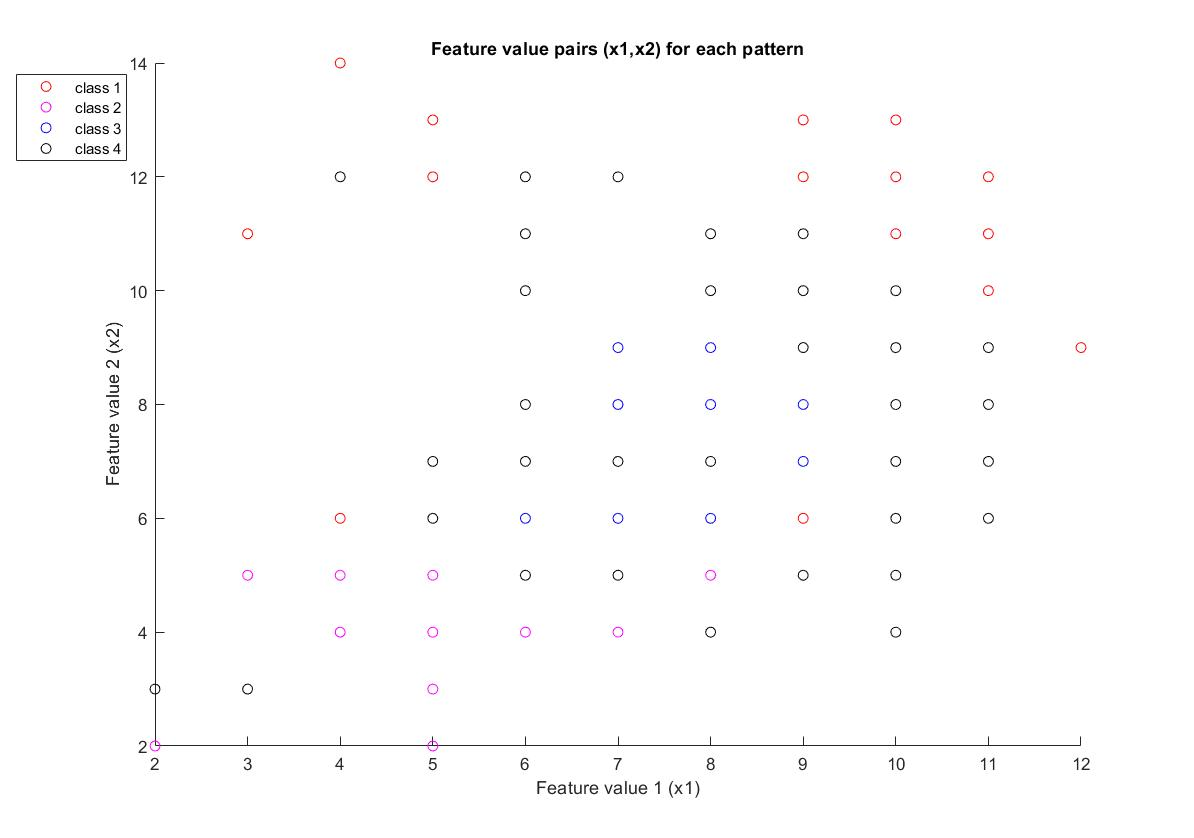
\includegraphics[scale=0.3]{q1pd_1.jpg}
\end{figure}
\pagebreak
\begin{figure}[H]
\centering
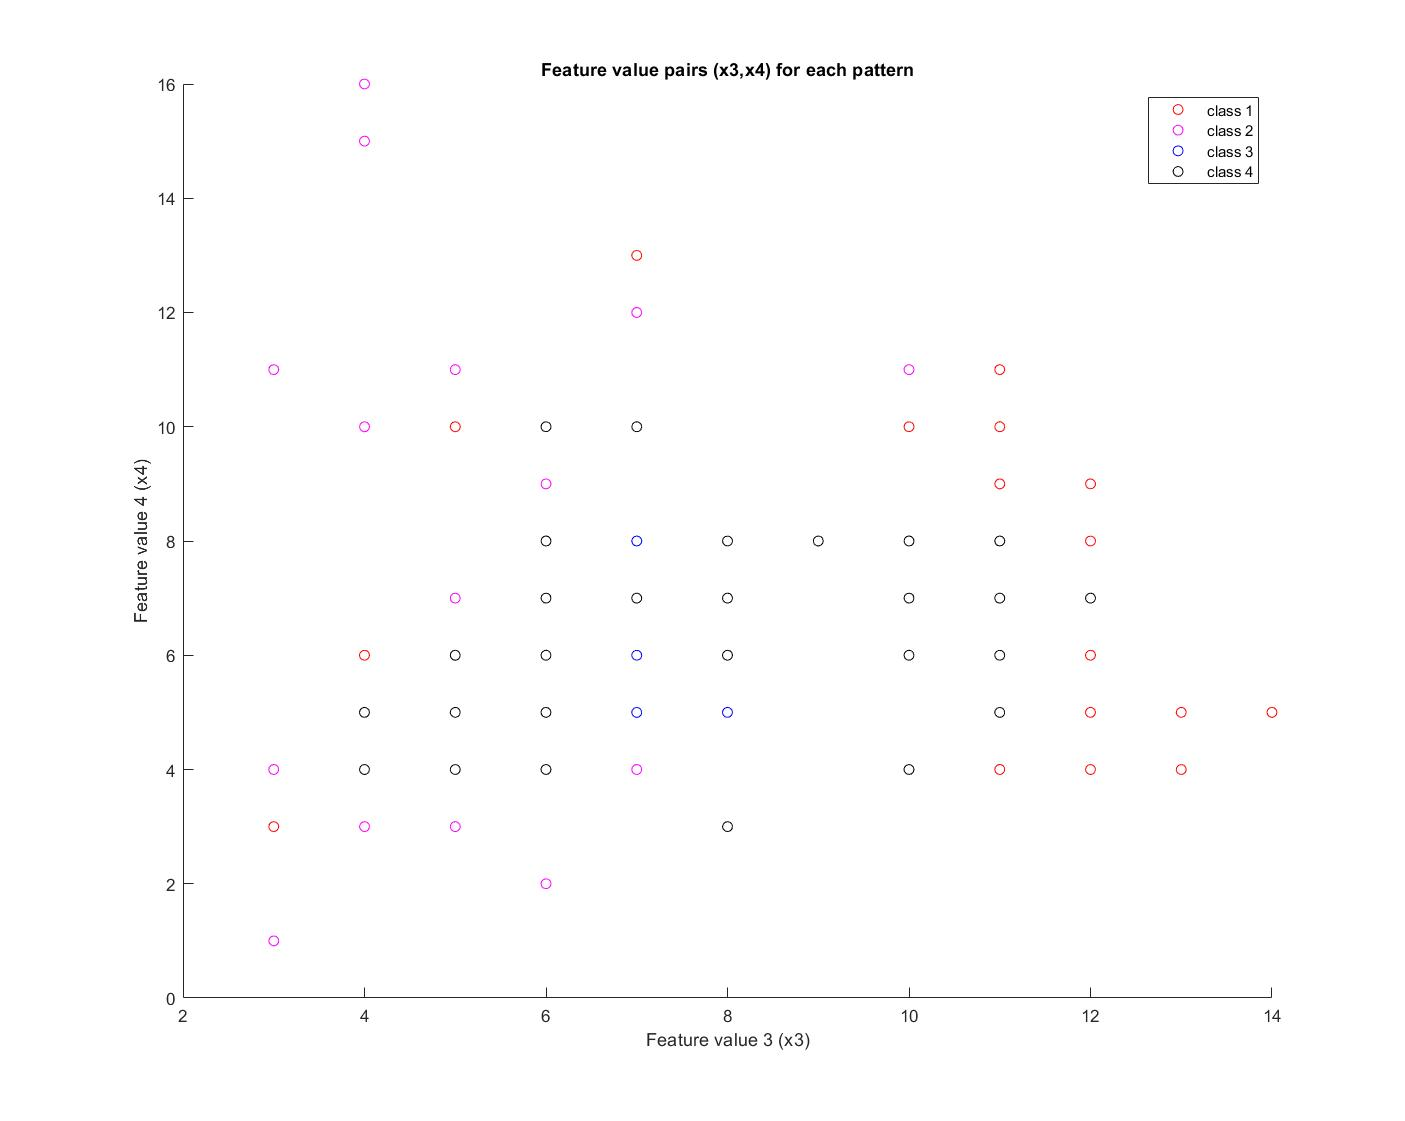
\includegraphics[scale=0.3]{q1pd_2.jpg}
\end{figure}

Both scatter plots are useful in distinguishing between the 4 classes. But, feature subset $(x_3,x_4)$ seems slightly better. In this scatter plot, note that class 1 is distinctly occuptied in the middle right and bottom right regions. Also, class 2 is distinctly occupied in the top left and bottom left. Class 3 and class 4 are harder to distinguish between, but it can be seen that class 3 is tightly distributed near the center of the plot. In contrast, in feature subset $(x_1,x_2)$ , class 3 and 4 are harder to distinguish between and overlap to a greater extent. So, it can be said that feature subset $(x_3,x_4)$ shows a relatively larger inter-class variability than feature subset $(x_1,x_2)$ and therefore is likely to be more useful for seperating the 4 classes.

\subsection*{Part e:}
\begin{figure}[H]
\centering
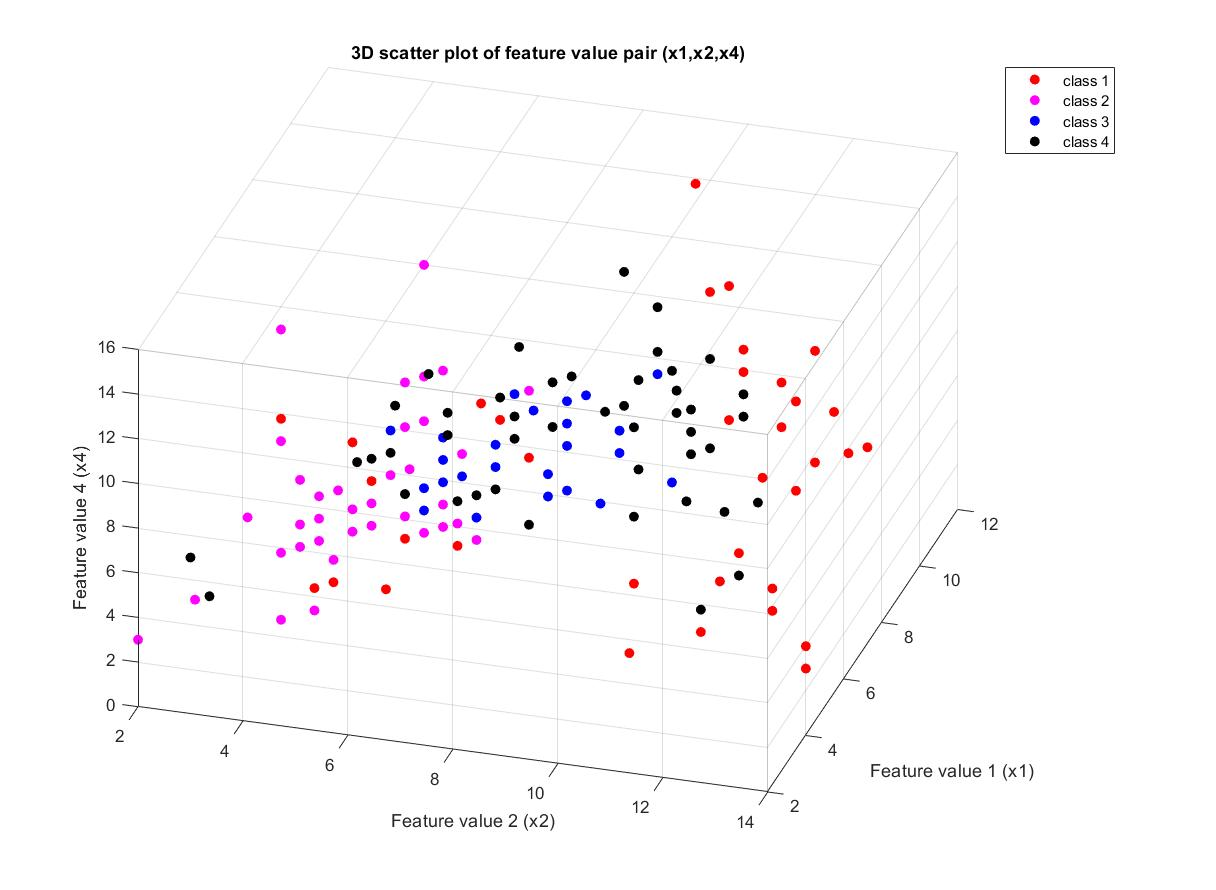
\includegraphics[scale=0.28]{q1pe.jpg}
\end{figure}
\begin{figure}[H]
\centering
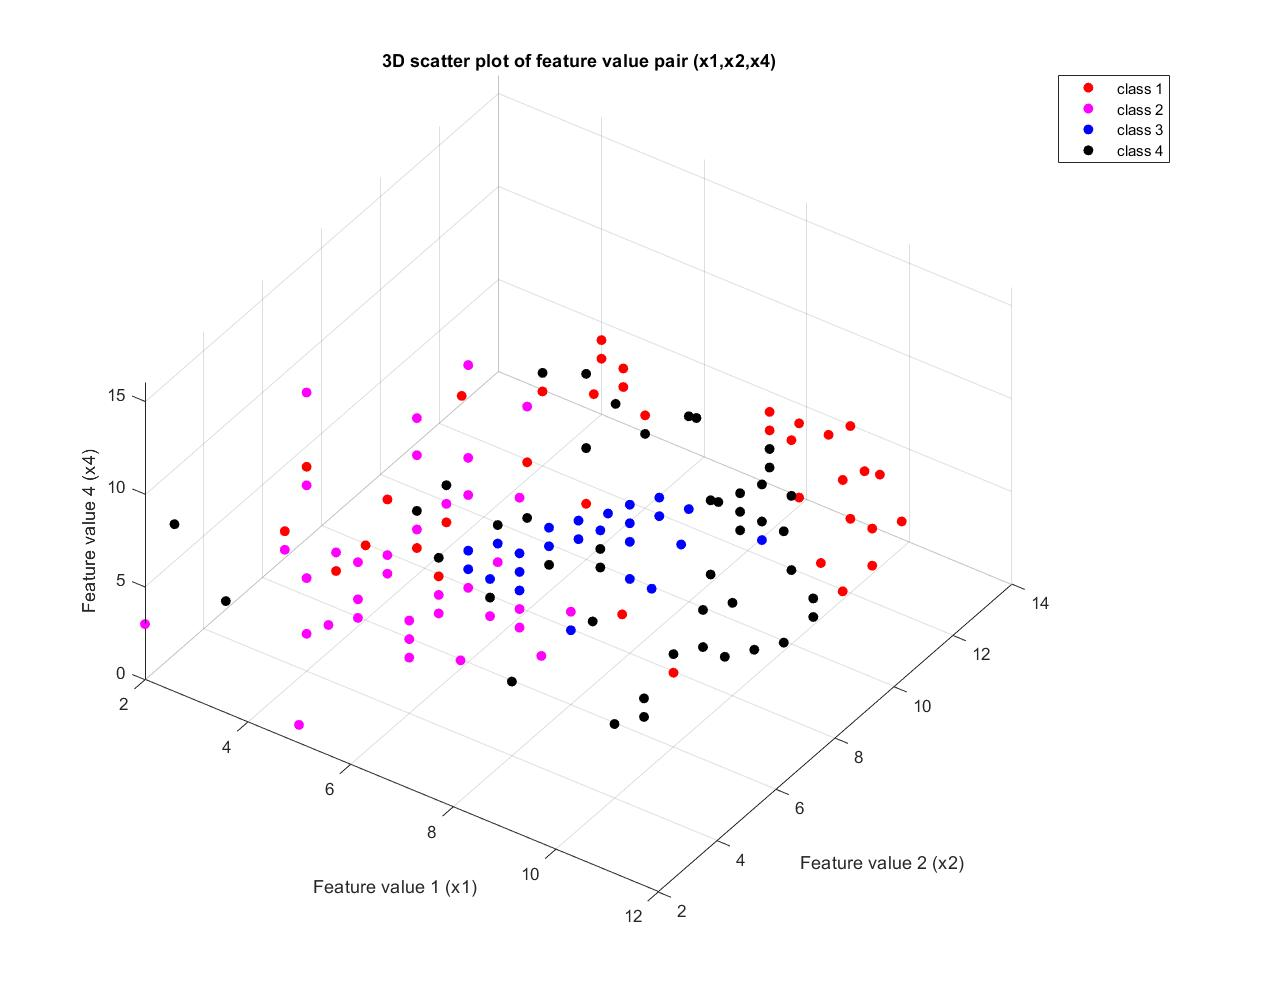
\includegraphics[scale=0.28]{q1pe_2.jpg}
\end{figure}
\pagebreak
It is difficult to determine which classes overlap each other. The 3D scatter plot in MATLAB allows us to view the plot at various angles. Class 3 and class 4 overlap to a great extent in the first image. This is especially prominent in the $(x_2,x_4)$ plane. Viewing from another angle, in the second image, we can also see that class 1 and class 2 overlap to a great extent in the $(x_1,x_2)$ plane.


\section*{Problem 2:}
\subsection*{Part a:}
Reinforcement learning is the ideal learning scheme for teaching a self-driving rover to navigate the terrain of Mars. The decisions involved for a self-driving rover is simple: drive over a given path or do not drive. This is at the core of reinforcement learning (learning with a critic), where there is no spefic desired category and the feedback is simply whether or not a classified category is right or wrong. Since it is unlikely for us to take into account the various terrain patterns in a foreign planet, labeleing patterns becomes a challenge. For this reason, supervised learning is not the best fit.

\subsection*{Part b:}
Unsupervised learning is the ideal leraning scheme for discovering a category of flowers given a large set of unknown flowers. Since the flowers are unknown, we cannot label them and supervised learning is not ideal. In unsupervised learning, there is no teacher and thefore classification is done implicitly via some sort of clustering. This clustering can be based on color, geometry, texture, and scent of flowers as described in the problem.

\subsection*{Part c:}
Supervised learning is the ideal learning scheme for identity detection based on voice. Assuming we know whose voice is associated with an identity in our training data, we can label the data accordingly. Therefore, supervised learning can be used to give feedback (as a teacher) on whether or not someone was classified correctly in comparison to their given label. 

\subsection*{Part d:}
Supervised learning is the ideal learning scheme for predicting weather in the next 24 hours based on the current weather conditions.  We do not need to rely on unsupervised learning since we have knowledge of current weather condiction. Our input data could consist of feature vectors pertaining to precipitation, humidity, temperature etc. and a label that specifies the outcome of the weather conditions after 24 hours (ex: snow, rain, wind etc.). We can provide this label (as teachers) in supervised learning.

\subsection*{Part e:}
Unsupervised learning is the ideal learning shceme for grouping similar looking faces together. The core of this problem is grouping or clustering. Unsupervised learning, as stated before, classifies implicitly based on clustering. Knowlegde of a face's identity isn't useful in determing whether or not that face is similar to a another face. Since it is challenging to "label" an area of traning, supervised learning is not ideal.

\section*{Problem 3:}
\subsection*{Part a:}
Overfitting is a phenomenon where a model fits the original tranining data well but does poorly against new/novel data. For example, let us consider the problem of classifying fish into salmon or sea bass, as discussed in lecture. Overfitting can occurs when we increase the complexity of the classifier too much. In this situation, our decision boundary between sea bass and salmon could be an 8th degree polynomial for example. While this boundary may fit the training data to a great extent, it doesn't generalize well and is poor at classifying new fish. In contrast, a simpler classifier such as a linear or quadratic one fits the training data adequetely but also adapts to novel data because it adequately captured the general trend for these 2 classes.

\subsection*{Part b:}
A loss function specifies the cost of an action to the model. A simple loss function may have an equal cost to every misclassified pattern, in which case the classification is based solely on the posterior probability and the priors. More complex loss functions can indicate the cost of misclassifying each class as every other class. This impacts the classifier such that the decision boundary relies on more than just the posterior probability. An obvious example can be found in the medical field. The cost of misdiagnosing a normal patient as having HIV is far cheaper than misdiagnosing a true HIV patient as normal. The latter could die from the mistake, whereas the former would incur monetary costs for unnecessary office visits and medications.  Therefore a simple loss function is not ideal in this case, and a more speific loss function would allow the model to classify to minimize the costs rather than minimizing error.

\subsection*{Part c:}
A decision boundary is a function that acts to seperate various classes. The boundary can be as simple as a line or as complex as a hyperplane, varying in polynomial complexity and/or dimensions. An example of a decision boundary is grading in school. The decision boundary at x = 0.9 (line) can seperate students with a 4.0 and students with 3.5 or below. In this example, the grades are the various classes. 

\subsection*{Part d:}
Segmentation is the process of isolating out the desired properties of a pattern and separating them out from undesired properties like background noise and other patterns. Segmentation is just one type of pattern pre-processing. For example, assume we are given the task to classify red blood cells based on their shape in a given image.  Segmentation might involve removing the background plasma from the image, and using color segmentation to seperate the red blood cells from neighboring white blood cells or proteins etc. Only once we have isoloated the red blood cells, we can move on to feature extraction.

\subsection*{Part e:}
Invariant represenation is the desired property that a given pattern is recognizable even if it was presented differently. For example, let us assme we are given the task to classify various objects based on their shape (cube, pyramid, sphere etc.) from our input data which consists of pictures of these shapes. We say that our data is an invariant representation if we process the data such that we can regonize a cube as such if even the camera took the picture closer than normal. This idea is specifically called scale invariance. After all, a cube should be recognized as a cube regardless of the distance between the camera and the object. Scale is just one type of invariance. Invariance can involve color, texture, etc.

\section*{Problem 4:}
\subsection*{Part a:}

\textbf{i)} This study used accelerometers and gyroscope sensors in cell phones to obtain two characterestics: acceleration and rotation. This is useful in measuring the intensity of physical activity by the participants.\\
\textbf{ii)} The data consists of a time series of collected 30 Hz sensory information for each activity done by each participant. Since the experiment involved the research staff manually toggling the recording device on and putting it on the participant's arm, the beginning and the end (researchers had to stop the device manually after data collection) of each time series was trimmed out.
\textbf{iii)} A total of 4 features were extracted in a sliding window of 2-seconds in size with a 1-second overlap between consecutive windows:
\begin{itemize}
  \item For each axis of acceleration, axis of rotation, and acceleration magnitude, the \textbf{mean} was calculated by the square root of the sum of each individual component squared: $\sqrt{A_x^2 + A_y^2 + A_z^2}$
  \item \textbf{Standard deviation} was calculated for axis of acceleration, axis of rotation, and acceleartion magnitude for each sliding window of time series.
\item \textbf{Sum} of acceleration magnitude
\item \textbf{Fast Fourier transform magnitude} - which is the magnitude of the first 5 coefficients of the Fourier transform power spectrum.
\end{itemize}
\textbf{iv)}
This study used the k-nearest neighbor classification scheme from the Waikato Environment for Knowledge Analysis (WEKA) machine learning tool kit. This learning scheme had the highest accurancy in comparison to decision tree, multiplayer preception, logistic, and naive Bayes. They then further boosted the classifier by applying AdaBoostM1 and bagging, but no clear benefits were observed.\\

In total there are 4 features per sample (60 samples) per activity (13 activities) per participant (16 participants) ${d = 4}$.
In total, there are 9 classes: slow walking, normal walking, brisk walking, jogging, sitting, normal upstairs, normal downstairs, brisk upstairs, and brist downstairs. ${c = 9}$

\subsection*{Part b:}
As described above, classifier training was accoplished by using the k-nearest neighbor, boosted by AdaBoostM1 and bagging via WEKA machine learning toolkit. Using the confusion matrix, summing the count in each cell gives us a total of 2807 patterns. Since not every participant was able to complete all activities, the number of patterns is lower than expected. Since the participant was aware of the activities they are performing, the patterns were labeled based upon the participant. 

\subsection*{Part c:}
Performance of the pattern recognition system was evaluated by comparing the classifed pattern with the original label. The number classified correctly was recorded and divided by the total number of patterns for each class, thereby obtaining classification accuracy for each class. \\
In terms of metrics used, the study compared classsification accuracy (as described above) using only acceleration  compared to using both acceleration and rotation. They also tested various window sizes (1 second, 2 seconds, 5 seconds, and 10 seconds), to determine that indeed 2-seconds had the highest overall accuracy.\\
They compared classification accuracy using k-nearest neighbor with decision tree, multilayer perception, logistic, naive Bayes, boosting, and bagging.\\
The study also compared classification accuracy from the current study to 3 studies in the past.

\subsection*{Part d:}
In my opinion, I believe the pattern recognition system performed well.  For at least half the classes, it had an accuracy of \textgreater 90 \%. Common categories such as sitting, walking, and jogging, were classified with high accurary. Activity involving stairs had lower accuracies but still performed better than prior studies. Though the study had limitations due to narrow demographics, fixed device placement, and small sample size, I believe the pattern recognition system performed well for the given task.

\section*{Problem 5:}
The probability density function is shown below:\\
${p(x) = K(x^3(10-x))}$ \\
Since we know that this is a probability density function, the area under the curve must equal 1. We are given the range is ${0 \leq x \leq 10}$ \\

\[\int_{0}^{10} K(x^3(10-x)) dx = 1\] 

\[K(\frac{10x^4}{4} -  \frac{x^5}{5})\Biggr|_0^{10} = 1\] 

\[K(\frac{10(10)^4}{4} -  \frac{10^5}{5} - 0) = 1\] 
\[5000K = 1\] 
\[K = \frac{1}{5000}\]

\section*{Problem 6:}
\subsection*{Part a:}
\begin{figure}[H]
\centering
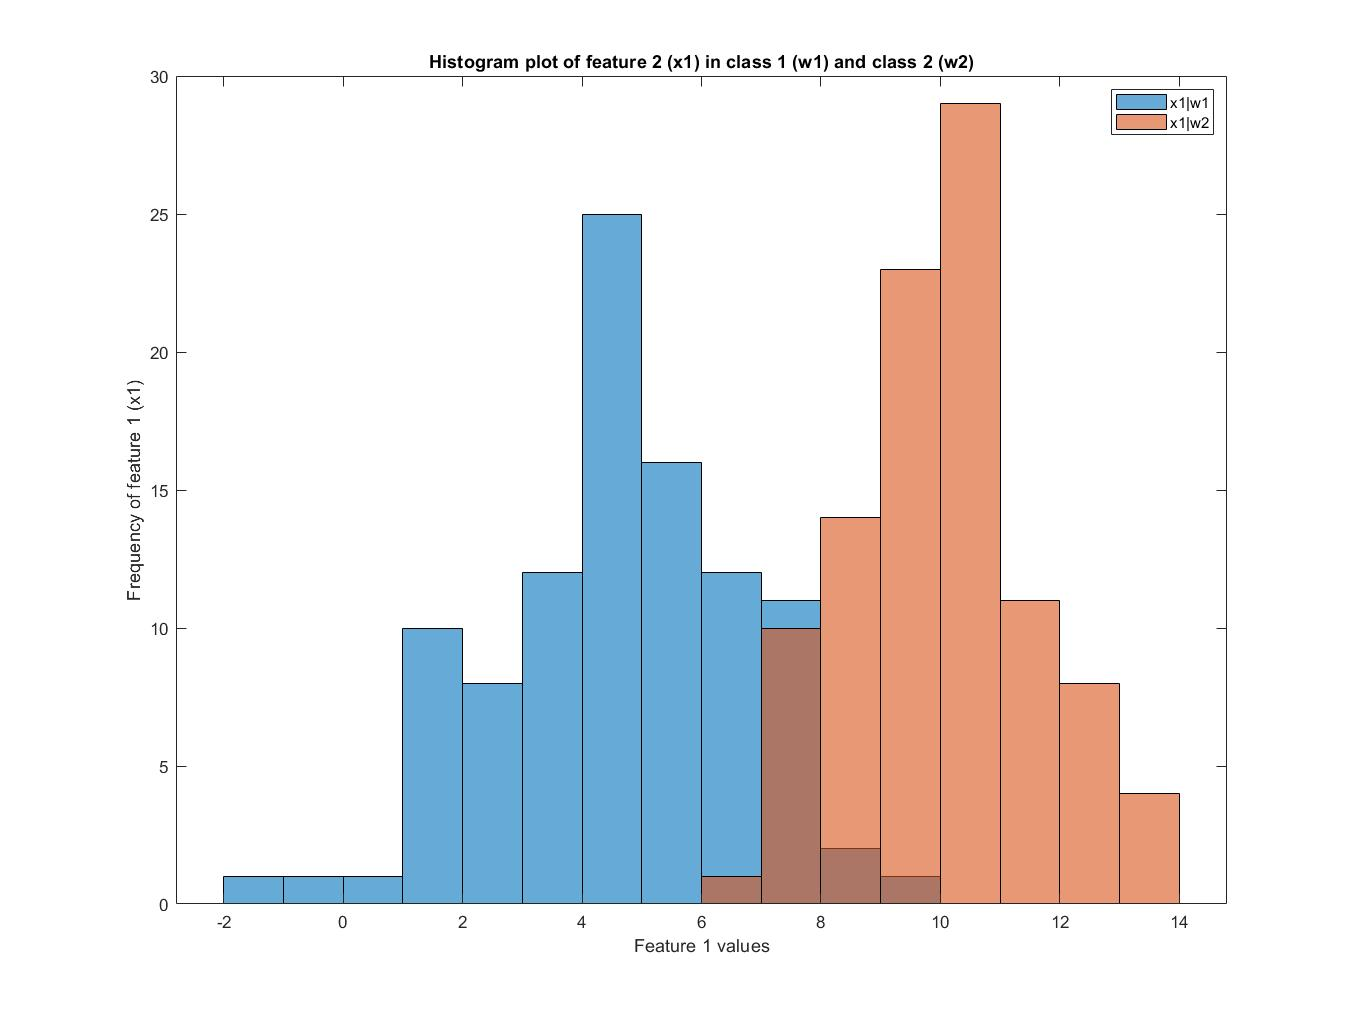
\includegraphics[scale=0.26]{q6pa_1.jpg}
\end{figure}
\pagebreak
\begin{figure}[H]
\centering
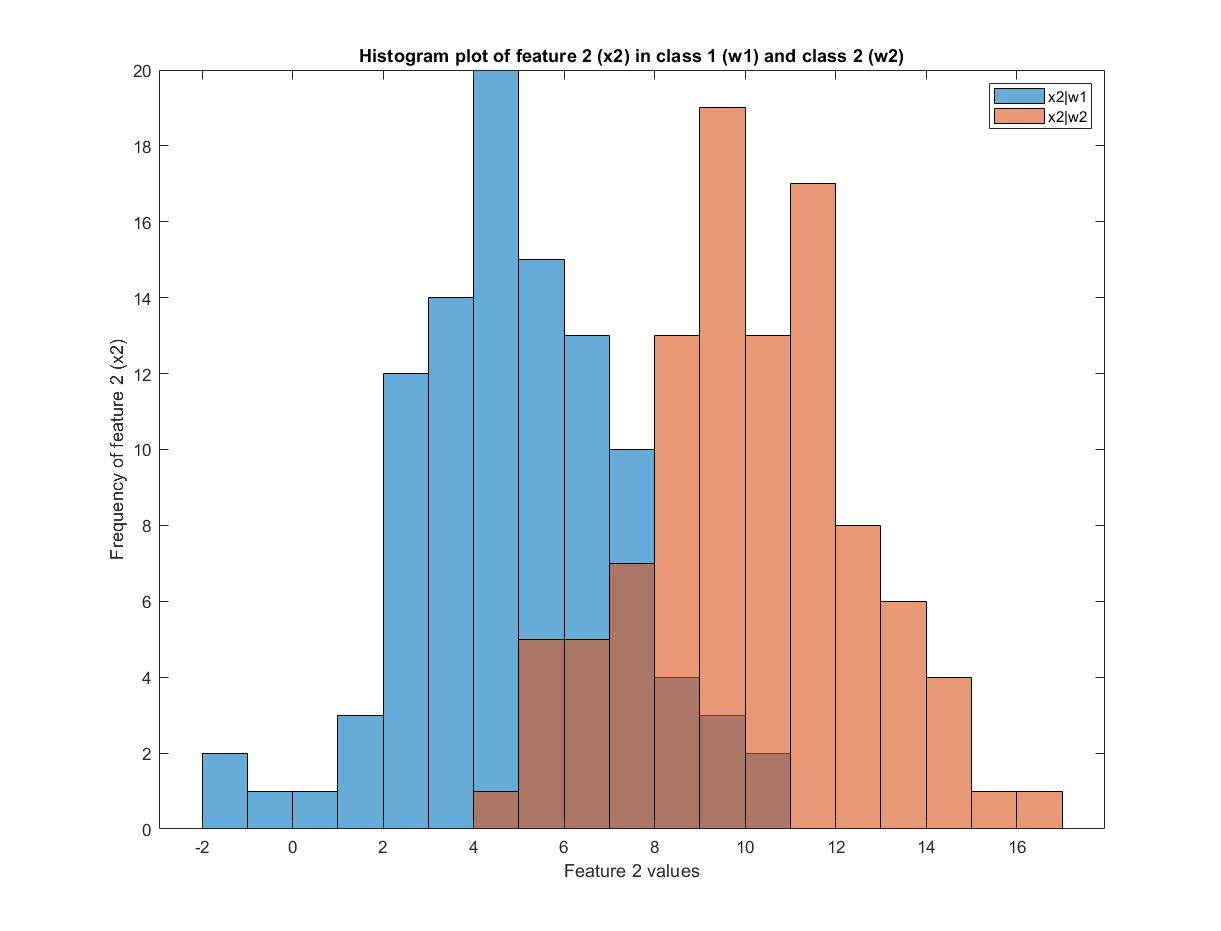
\includegraphics[scale=0.26]{q6pa_2.jpg}
\end{figure}

As seen from the above images, $x_1$ is more discriminatory than $x_2$. There is far less overlap between $(x_1|w_1)$ and $(x_1|w_2)$ when compared to $(x_2|w_1)$ and $(x_2|w_2)$.

\subsection*{Part b:}
\begin{figure}[H]
\centering
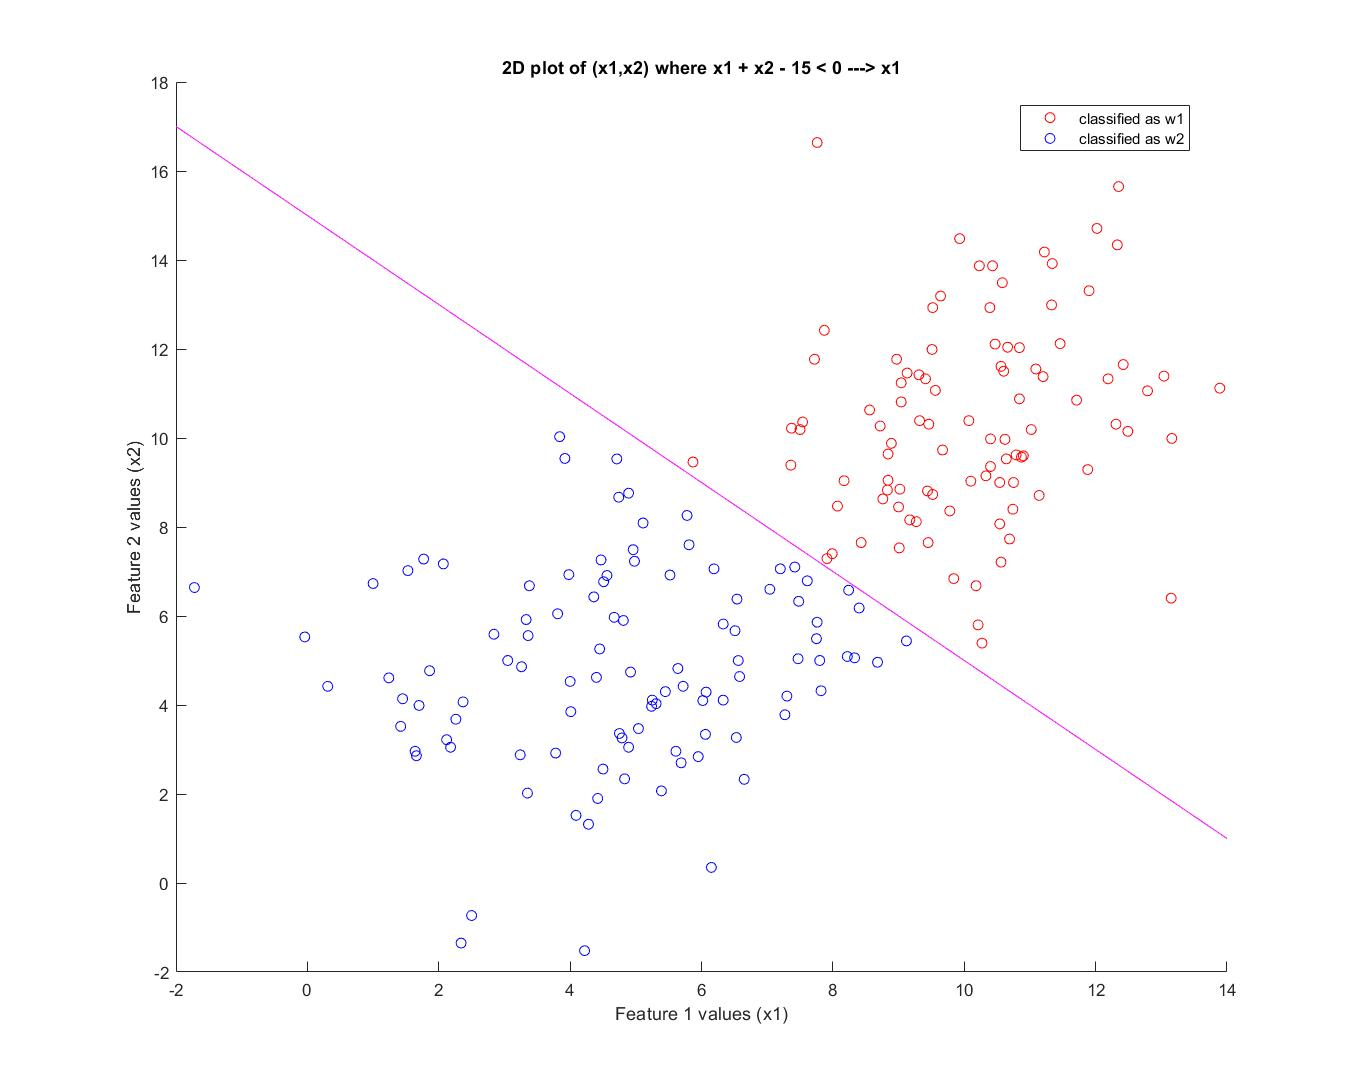
\includegraphics[scale=0.22]{q6pb.jpg}
\end{figure}

The decision boundary $x_1 + x_2 - 15 < 0$, $x$ $\epsilon$ $\omega_1$ else $x$ $\epsilon$ $\omega_2$ is plotted as a magenta line in the plot above. Using MATLAB, the number of patterns misclassified by this boundary is exactly 10. Since there are 200 patterns in total, the error rate is $\frac{10}{200} = 0.05 = 5 \%$

\subsection*{Part c:}
\begin{figure}[H]
\centering
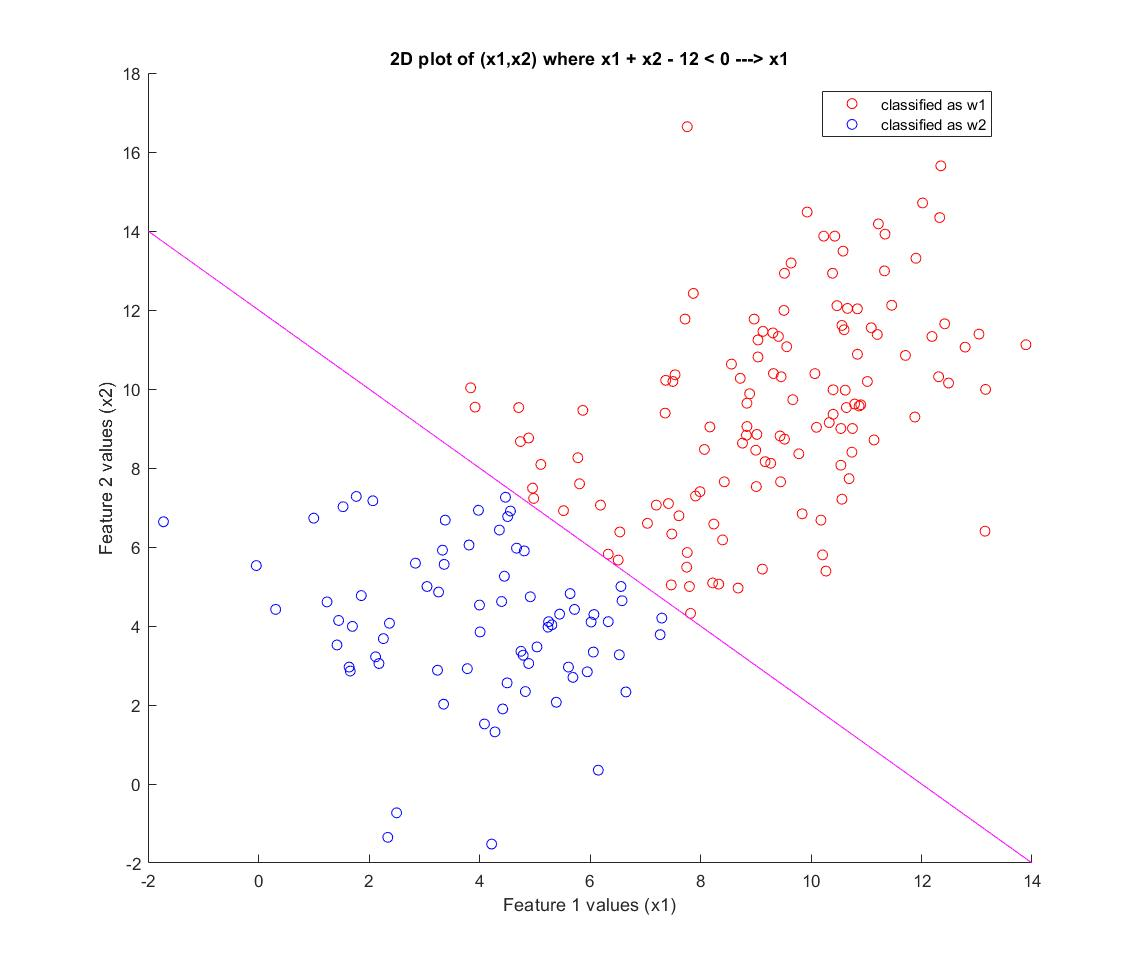
\includegraphics[scale=0.23]{q6pc.jpg}
\end{figure}

The decision boundary $x_1 + x_2 - 12 < 0$, $x$ $\epsilon$ $\omega_1$ else $x$ $\epsilon$ $\omega_2$ is plotted as a magenta line in the plot above. Using MATLAB, the number of patterns misclassified by this boundary is exactly 27. Since there are 200 patterns in total, the error rate is $\frac{27}{200} = 0.135 = 13.5 \%$

\subsection*{Part d:}
From looking at the error rate between the two classifier, it is clear that the first classifier performed better on this dataset.  The first classifier only had an error of 5\%, wheras the second had an error of 13.5\%. Therefore, it is clear that $x_1 + x_2 - 15 < 0$, $x$ $\epsilon$ $\omega_1$ else $x$ $\epsilon$ $\omega_2$ is the better decision boundary (classifier).
\pagebreak
\section*{Appendix:}
Here is the code I used during the homework:
\begin{figure}[H]

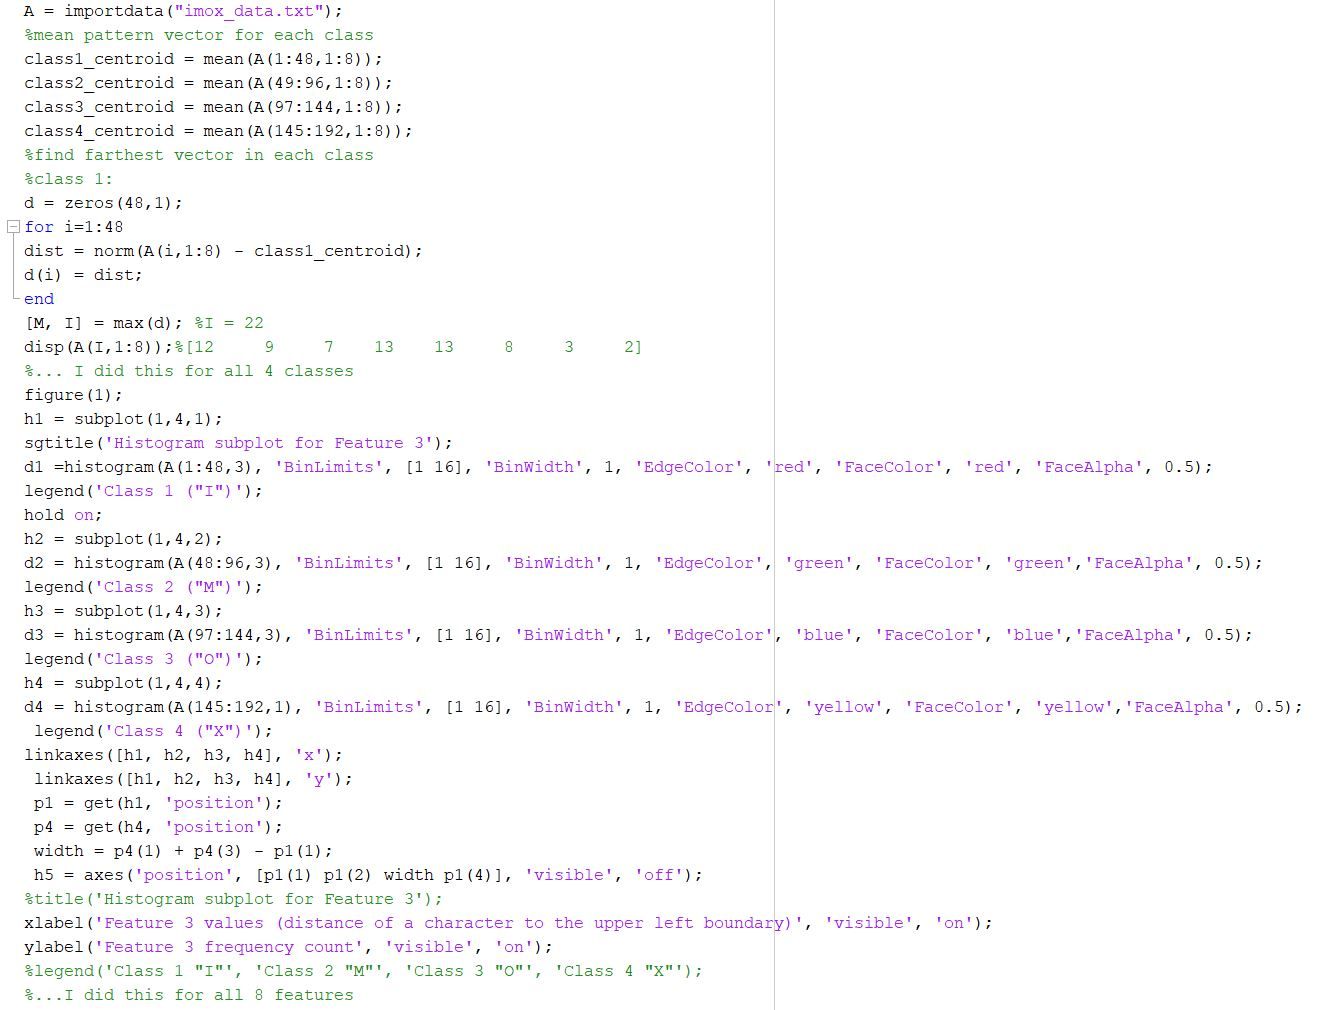
\includegraphics[scale=0.48]{matlab_code_1.jpg}
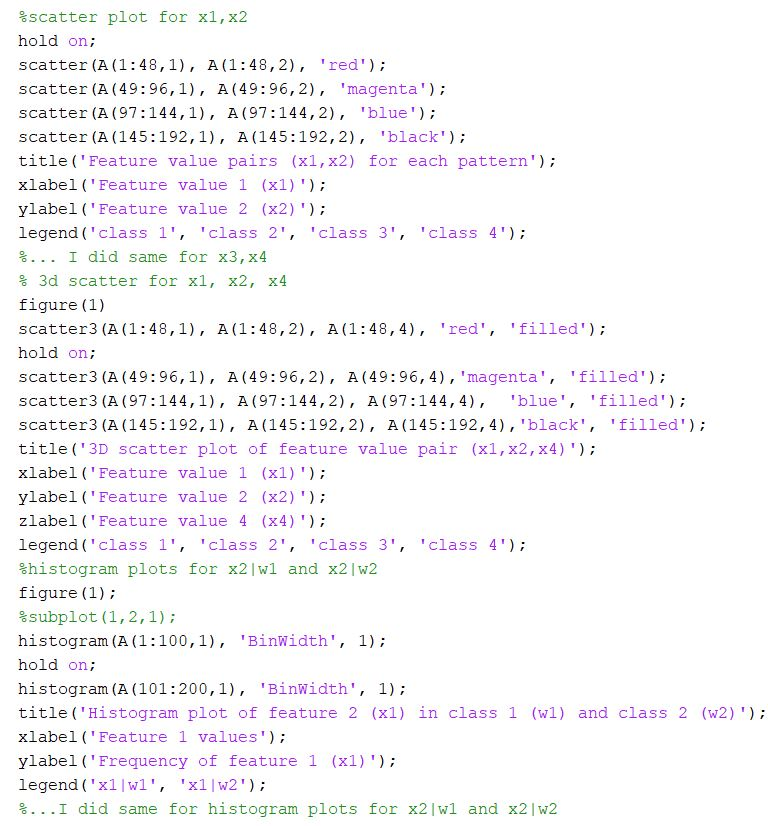
\includegraphics[scale=0.48]{matlab_code_2.jpg}
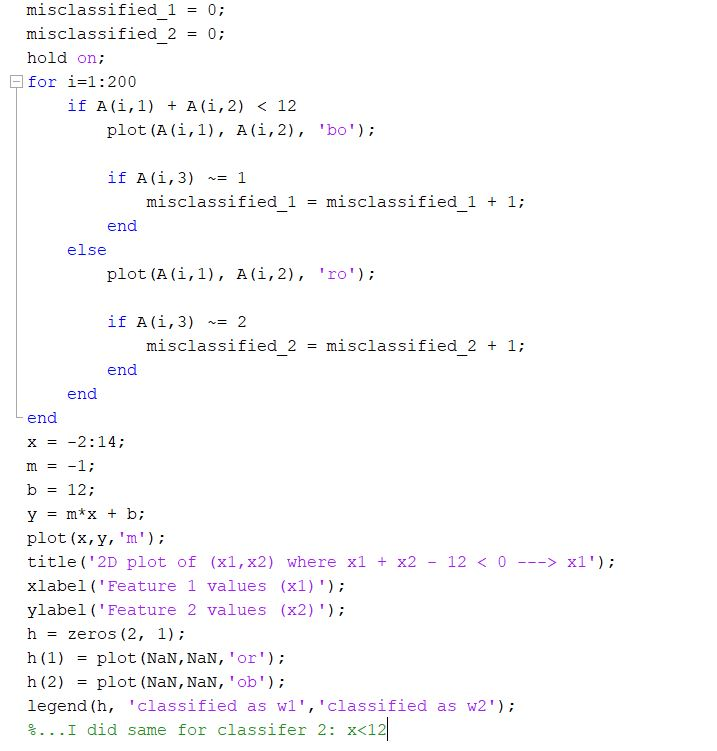
\includegraphics[scale=0.48]{matlab_code_3.jpg}
\end{figure}



\end{document}